
%\VignetteEngine{knitr::knitr}
%\VignetteIndexEntry{mtram}
%\VignetteDepends{variables, basefun, mlt, tram, survival, lme4, gridExtra, lattice, latticeExtra, colorspace, HSAUR3, mvtnorm, ordinalCont, tramME}

\documentclass[article,nojss,shortnames]{jss}\usepackage[]{graphicx}\usepackage[]{xcolor}
% maxwidth is the original width if it is less than linewidth
% otherwise use linewidth (to make sure the graphics do not exceed the margin)
\makeatletter
\def\maxwidth{ %
  \ifdim\Gin@nat@width>\linewidth
    \linewidth
  \else
    \Gin@nat@width
  \fi
}
\makeatother





%% packages
\usepackage{thumbpdf}
\usepackage{amsfonts,amstext,amsmath,amssymb,amsthm}
\usepackage{accents}
\usepackage{color}
\usepackage{rotating}
\usepackage{verbatim}
\usepackage[utf8]{inputenc}
%% need no \usepackage{Sweave.sty}
%%\usepackage[nolists]{endfloat}

\newcommand{\cmd}[1]{\texttt{#1()}}


\usepackage{tikz}
\usetikzlibrary{shapes,arrows,chains}
\usepackage{verbatim}



\newcommand{\TODO}[1]{{\color{red} #1}}

\newcommand\Torsten[1]{{\color{blue}Torsten: ``#1''}}

\newcommand{\THcite}[2]{\citeauthor{#2} (\citeyear{#2})}


\newcommand\norm[1]{\left\lVert#1\right\rVert}

\newcommand{\CTM}{CTM Likelihood Boosting}
\newcommand{\STM}{STM Likelihood Boosting}

\newcommand{\etc}{\textit{etc.}}

\usepackage{booktabs}

\newcommand{\expit}{\text{expit}}

%%% mlt
%% rv
\newcommand{\rZ}{Z}
\newcommand{\rY}{Y}
\newcommand{\rX}{\mX}
\newcommand{\rz}{z}
\newcommand{\ry}{y}
\newcommand{\rx}{\xvec}
\newcommand{\ru}{\uvec}
\newcommand{\erx}{x}
%% sigma algebra
\newcommand{\sA}{\mathfrak{A}}
\newcommand{\sAZ}{\mathfrak{B}}
\newcommand{\sAY}{\mathfrak{C}}
\newcommand{\esA}{A}
\newcommand{\esAZ}{B}
\newcommand{\esAY}{C}
%% sample spaces
\newcommand{\sam}{\Omega}
\newcommand{\samZ}{\RR}
\newcommand{\samY}{\Xi}
\newcommand{\samX}{\chi}
%% measureable spaces
\newcommand{\ms}{(\sam, \sA)}
\newcommand{\msZ}{(\samZ, \sAZ)}
\newcommand{\msY}{(\samY, \sAY)}
%% probability spaces
\newcommand{\ps}{(\sam, \sA, \Prob)}
\newcommand{\psZ}{(\samZ, \sAZ, \Prob_\rZ)}
\newcommand{\psY}{(\samY, \sAY, \Prob_\rY)}
%% distributions
\newcommand{\pZ}{F}
\newcommand{\pY}{F_\rY}
\newcommand{\oY}{O_\rY}
\newcommand{\oYx}{O_{\rY \mid \rX = \rx}}
\newcommand{\hatpY}{\hat{F}_{\rY,N}}
\newcommand{\hatpYx}{\hat{F}_{\rY \mid \rX = \rx, N}}
\newcommand{\PYx}{\Prob_{\rY \mid \rX = \rx}}
\newcommand{\PYX}{\Prob_{\rY, \rX}}
\newcommand{\PY}{\Prob_{\rY}}
\newcommand{\pN}{\Phi}
\newcommand{\pSL}{F_{\SL}}
\newcommand{\pMEV}{F_{\MEV}}
\newcommand{\pExp}{F_{\ExpD}}
\newcommand{\pSW}{F_{\SW}}
\newcommand{\pYx}{F_{\rY \mid \rX = \rx}}
\newcommand{\pYA}{F_{\rY \mid \rX = A}}
\newcommand{\pYB}{F_{\rY \mid \rX = B}}
\newcommand{\qZ}{F^{-1}_\rZ}
\newcommand{\qY}{F^{-1}_\rY}
\newcommand{\dZ}{f}
\newcommand{\dY}{f_\rY}
\newcommand{\hatdY}{\hat{f}_{\rY, N}}
\newcommand{\dYx}{f_{\rY \mid \rX = \rx}}
\newcommand{\hazY}{\lambda_\rY}
\newcommand{\HazY}{\Lambda_\rY}
\newcommand{\HazYx}{\Lambda_{\rY \mid \rX = \rx}}

\newcommand{\hathazY}{\hat{\lambda}_{\rY, N}}
\newcommand{\hatHazY}{\hat{\Lambda}_{\rY, N}}
%% measures
\newcommand{\measureY}{\mu}
\newcommand{\lebesgue}{\mu_L}
\newcommand{\counting}{\mu_C}
%% trafo
\newcommand{\g}{g}
\newcommand{\h}{h}
\newcommand{\s}{\svec}
\newcommand{\hY}{h_\rY}
\newcommand{\hx}{h_\rx}
\newcommand{\hs}{\mathcal{H}}
\newcommand{\basisy}{\avec}
\newcommand{\bern}[1]{\avec_{\text{Bs},#1}}
\newcommand{\bernx}[1]{\bvec_{\text{Bs},#1}}
\newcommand{\basisx}{\bvec}
\newcommand{\basisyx}{\cvec}
\newcommand{\m}{m}
\newcommand{\lik}{\mathcal{L}}
\newcommand{\parm}{\varthetavec}
\newcommand{\eparm}{\vartheta}
\newcommand{\dimparm}{P}
\newcommand{\dimparmx}{Q}
\newcommand{\dimparmvar}{M}
\newcommand{\dimparmrand}{R}
\newcommand{\shiftparm}{\betavec}
\newcommand{\scaleparm}{\xivec}
\newcommand{\varparm}{\gammavec}
\newcommand{\eshiftparm}{\beta}
\newcommand{\escaleparm}{\xi}

\newcommand{\ie}{\textit{i.e.}~}
\newcommand{\eg}{\textit{e.g.}~}

\renewcommand{\Prob}{\mathbb{P}}
\newcommand{\Ex}{\mathbb{E}}
\newcommand{\RR}{\mathbb{R}}
\newcommand{\NN}{\mathbb{N}}
\newcommand{\eps}{\varepsilon}
\newcommand{\prodname}{tensor }
\newcommand{\Null}{\mathbf{0}}
\newcommand{\FI}{\mF}

\usepackage{dsfont}
\newcommand{\I}{\mathds{1}}



\def \dsP {\text{$\mathds{P}$}}
\def \dsE {\text{$\mathds{E}$}}
\def \dsR {\text{$\mathds{R}$}}
\def \dsN {\text{$\mathds{N}$}}


% Math Operators

 \DeclareMathOperator{\logit}{logit}
 \DeclareMathOperator{\LRT}{LRT}
 \DeclareMathOperator{\RLRT}{RLRT}
 \DeclareMathOperator{\Cov}{Cov}
 \DeclareMathOperator{\Cor}{Cor}
 \DeclareMathOperator{\Var}{Var}
 \DeclareMathOperator{\EW}{\dsE}
 \DeclareMathOperator{\D}{D}
 \DeclareMathOperator{\Bias}{Bias}
 \DeclareMathOperator{\MSE}{MSE}
 \DeclareMathOperator{\PLS}{PLS}
 \DeclareMathOperator{\rank}{rank}
 \DeclareMathOperator{\ncol}{ncol}
 \DeclareMathOperator{\pen}{pen}
 \DeclareMathOperator{\const}{const}
 \DeclareMathOperator{\diag}{diag}
 \DeclareMathOperator{\blockdiag}{blockdiag}
 \DeclareMathOperator{\df}{df}
 \DeclareMathOperator{\trace}{tr}
 \DeclareMathOperator{\iid}{i.i.d.}
 \DeclareMathOperator{\ind}{ind.}
 \DeclareMathOperator{\obs}{obs}
 \DeclareMathOperator{\acos}{acos}
 \DeclareMathOperator{\spat}{spat}
 \DeclareMathOperator{\fix}{{fix}}
 \DeclareMathOperator{\ran}{{ran}}
 \DeclareMathOperator*{\argmin}{{arg\,min}}
 \DeclareMathOperator*{\argmax}{{arg\,max}}
 \DeclareMathOperator{\BIC}{{BIC}}
 \DeclareMathOperator{\DIC}{{DIC}}
 \DeclareMathOperator{\AIC}{{AIC}}
 \DeclareMathOperator{\mAIC}{{mAIC}}
 \DeclareMathOperator{\cAIC}{{cAIC}}

% Distributions

 \DeclareMathOperator{\ND}{N}
 \DeclareMathOperator{\TND}{TN}
 \DeclareMathOperator{\UD}{U}
 \DeclareMathOperator{\GaD}{Ga}
 \DeclareMathOperator{\tD}{t}
 \DeclareMathOperator{\IGD}{IG}
 \DeclareMathOperator{\IWD}{IW}
 \DeclareMathOperator{\PoD}{Po}
 \DeclareMathOperator{\ExpD}{Exp}
 \DeclareMathOperator{\LapD}{Lap}
 \DeclareMathOperator{\MuD}{Mu}
 \DeclareMathOperator{\DirD}{Dir}
 \DeclareMathOperator{\PDD}{PD}
 \DeclareMathOperator{\BeD}{Be}
 \DeclareMathOperator{\BD}{B}
 \DeclareMathOperator{\DPD}{DP}
 \DeclareMathOperator{\KSD}{KS}
 \DeclareMathOperator{\SL}{SL}
 \DeclareMathOperator{\MEV}{MEV}
 \DeclareMathOperator{\SW}{SW}
 \DeclareMathOperator{\Chi1}{\chi^2_1}
 \DeclareMathOperator{\WD}{W}



% Boldface vectors and matrices

\def \avec {\text{\boldmath$a$}}    \def \mA {\text{\boldmath$A$}}
\def \bvec {\text{\boldmath$b$}}    \def \mB {\text{\boldmath$B$}}
\def \cvec {\text{\boldmath$c$}}    \def \mC {\text{\boldmath$C$}}
\def \dvec {\text{\boldmath$d$}}    \def \mD {\text{\boldmath$D$}}
\def \evec {\text{\boldmath$e$}}    \def \mE {\text{\boldmath$E$}}
\def \fvec {\text{\boldmath$f$}}    \def \mF {\text{\boldmath$F$}}
\def \gvec {\text{\boldmath$g$}}    \def \mG {\text{\boldmath$G$}}
\def \hvec {\text{\boldmath$h$}}    \def \mH {\text{\boldmath$H$}}
\def \ivec {\text{\boldmath$i$}}    \def \mI {\text{\boldmath$I$}}
\def \jvec {\text{\boldmath$j$}}    \def \mJ {\text{\boldmath$J$}}
\def \kvec {\text{\boldmath$k$}}    \def \mK {\text{\boldmath$K$}}
\def \lvec {\text{\boldmath$l$}}    \def \mL {\text{\boldmath$L$}}
\def \mvec {\text{\boldmath$m$}}    \def \mM {\text{\boldmath$M$}}
\def \nvec {\text{\boldmath$n$}}    \def \mN {\text{\boldmath$N$}}
\def \ovec {\text{\boldmath$o$}}    \def \mO {\text{\boldmath$O$}}
\def \pvec {\text{\boldmath$p$}}    \def \mP {\text{\boldmath$P$}}
\def \qvec {\text{\boldmath$q$}}    \def \mQ {\text{\boldmath$Q$}}
\def \rvec {\text{\boldmath$r$}}    \def \mR {\text{\boldmath$R$}}
\def \svec {\text{\boldmath$s$}}    \def \mS {\text{\boldmath$S$}}
\def \tvec {\text{\boldmath$t$}}    \def \mT {\text{\boldmath$T$}}
\def \uvec {\text{\boldmath$u$}}    \def \mU {\text{\boldmath$U$}}
\def \vvec {\text{\boldmath$v$}}    \def \mV {\text{\boldmath$V$}}
\def \wvec {\text{\boldmath$w$}}    \def \mW {\text{\boldmath$W$}}
\def \xvec {\text{\boldmath$x$}}    \def \mX {\text{\boldmath$X$}}
\def \yvec {\text{\boldmath$y$}}    \def \mY {\text{\boldmath$Y$}}
\def \zvec {\text{\boldmath$z$}}    \def \mZ {\text{\boldmath$Z$}}

 \def \calA {\mathcal A}
 \def \calB {\mathcal B}
 \def \calC {\mathcal C}
 \def \calD {\mathcal D}
 \def \calE {\mathcal E}
 \def \calF {\mathcal F}
 \def \calG {\mathcal G}
 \def \calH {\mathcal H}
 \def \calI {\mathcal I}
 \def \calJ {\mathcal J}
 \def \calK {\mathcal K}
 \def \calL {\mathcal L}
 \def \calM {\mathcal M}
 \def \calN {\mathcal N}
 \def \calO {\mathcal O}
 \def \calP {\mathcal P}
 \def \calQ {\mathcal Q}
 \def \calR {\mathcal R}
 \def \calS {\mathcal S}
 \def \calT {\mathcal T}
 \def \calU {\mathcal U}
 \def \calV {\mathcal V}
 \def \calW {\mathcal W}
 \def \calX {\mathcal X}
 \def \calY {\mathcal Y}
 \def \calZ {\mathcal Z}

\def \ahatvec {\text{\boldmath$\hat a$}}    \def \mhatA {\text{\boldmath$\hat A$}}
\def \bhatvec {\text{\boldmath$\hat b$}}    \def \mhatB {\text{\boldmath$\hat B$}}
\def \chatvec {\text{\boldmath$\hat c$}}    \def \mhatC {\text{\boldmath$\hat C$}}
\def \dhatvec {\text{\boldmath$\hat d$}}    \def \mhatD {\text{\boldmath$\hat D$}}
\def \ehatvec {\text{\boldmath$\hat e$}}    \def \mhatE {\text{\boldmath$\hat E$}}
\def \fhatvec {\text{\boldmath$\hat f$}}    \def \mhatF {\text{\boldmath$\hat F$}}
\def \ghatvec {\text{\boldmath$\hat g$}}    \def \mhatG {\text{\boldmath$\hat G$}}
\def \hhatvec {\text{\boldmath$\hat h$}}    \def \mhatH {\text{\boldmath$\hat H$}}
\def \ihatvec {\text{\boldmath$\hat i$}}    \def \mhatI {\text{\boldmath$\hat I$}}
\def \jhatvec {\text{\boldmath$\hat j$}}    \def \mhatJ {\text{\boldmath$\hat J$}}
\def \khatvec {\text{\boldmath$\hat k$}}    \def \mhatK {\text{\boldmath$\hat K$}}
\def \lhatvec {\text{\boldmath$\hat l$}}    \def \mhatL {\text{\boldmath$\hat L$}}
\def \mhatvec {\text{\boldmath$\hat m$}}    \def \mhatM {\text{\boldmath$\hat M$}}
\def \nhatvec {\text{\boldmath$\hat n$}}    \def \mhatN {\text{\boldmath$\hat N$}}
\def \ohatvec {\text{\boldmath$\hat o$}}    \def \mhatO {\text{\boldmath$\hat O$}}
\def \phatvec {\text{\boldmath$\hat p$}}    \def \mhatP {\text{\boldmath$\hat P$}}
\def \qhatvec {\text{\boldmath$\hat q$}}    \def \mhatQ {\text{\boldmath$\hat Q$}}
\def \rhatvec {\text{\boldmath$\hat r$}}    \def \mhatR {\text{\boldmath$\hat R$}}
\def \shatvec {\text{\boldmath$\hat s$}}    \def \mhatS {\text{\boldmath$\hat S$}}
\def \thatvec {\text{\boldmath$\hat t$}}    \def \mhatT {\text{\boldmath$\hat T$}}
\def \uhatvec {\text{\boldmath$\hat u$}}    \def \mhatU {\text{\boldmath$\hat U$}}
\def \vhatvec {\text{\boldmath$\hat v$}}    \def \mhatV {\text{\boldmath$\hat V$}}
\def \whatvec {\text{\boldmath$\hat w$}}    \def \mhatW {\text{\boldmath$\hat W$}}
\def \xhatvec {\text{\boldmath$\hat x$}}    \def \mhatX {\text{\boldmath$\hat X$}}
\def \yhatvec {\text{\boldmath$\hat y$}}    \def \mhatY {\text{\boldmath$\hat Y$}}
\def \zhatvec {\text{\boldmath$\hat z$}}    \def \mhatZ {\text{\boldmath$\hat Z$}}


\def \atildevec {\text{\boldmath$\tilde a$}}    \def \mtildeA {\text{\boldmath$\tilde A$}}
\def \btildevec {\text{\boldmath$\tilde b$}}    \def \mtildeB {\text{\boldmath$\tilde B$}}
\def \ctildevec {\text{\boldmath$\tilde c$}}    \def \mtildeC {\text{\boldmath$\tilde C$}}
\def \dtildevec {\text{\boldmath$\tilde d$}}    \def \mtildeD {\text{\boldmath$\tilde D$}}
\def \etildevec {\text{\boldmath$\tilde e$}}    \def \mtildeE {\text{\boldmath$\tilde E$}}
\def \ftildevec {\text{\boldmath$\tilde f$}}    \def \mtildeF {\text{\boldmath$\tilde F$}}
\def \gtildevec {\text{\boldmath$\tilde g$}}    \def \mtildeG {\text{\boldmath$\tilde G$}}
\def \htildevec {\text{\boldmath$\tilde h$}}    \def \mtildeH {\text{\boldmath$\tilde H$}}
\def \itildevec {\text{\boldmath$\tilde i$}}    \def \mtildeI {\text{\boldmath$\tilde I$}}
\def \jtildevec {\text{\boldmath$\tilde j$}}    \def \mtildeJ {\text{\boldmath$\tilde J$}}
\def \ktildevec {\text{\boldmath$\tilde k$}}    \def \mtildeK {\text{\boldmath$\tilde K$}}
\def \ltildevec {\text{\boldmath$\tilde l$}}    \def \mtildeL {\text{\boldmath$\tilde L$}}
\def \mtildevec {\text{\boldmath$\tilde m$}}    \def \mtildeM {\text{\boldmath$\tilde M$}}
\def \ntildevec {\text{\boldmath$\tilde n$}}    \def \mtildeN {\text{\boldmath$\tilde N$}}
\def \otildevec {\text{\boldmath$\tilde o$}}    \def \mtildeO {\text{\boldmath$\tilde O$}}
\def \ptildevec {\text{\boldmath$\tilde p$}}    \def \mtildeP {\text{\boldmath$\tilde P$}}
\def \qtildevec {\text{\boldmath$\tilde q$}}    \def \mtildeQ {\text{\boldmath$\tilde Q$}}
\def \rtildevec {\text{\boldmath$\tilde r$}}    \def \mtildeR {\text{\boldmath$\tilde R$}}
\def \stildevec {\text{\boldmath$\tilde s$}}    \def \mtildeS {\text{\boldmath$\tilde S$}}
\def \ttildevec {\text{\boldmath$\tilde t$}}    \def \mtildeT {\text{\boldmath$\tilde T$}}
\def \utildevec {\text{\boldmath$\tilde u$}}    \def \mtildeU {\text{\boldmath$\tilde U$}}
\def \vtildevec {\text{\boldmath$\tilde v$}}    \def \mtildeV {\text{\boldmath$\tilde V$}}
\def \wtildevec {\text{\boldmath$\tilde w$}}    \def \mtildeW {\text{\boldmath$\tilde W$}}
\def \xtildevec {\text{\boldmath$\tilde x$}}    \def \mtildeX {\text{\boldmath$\tilde X$}}
\def \ytildevec {\text{\boldmath$\tilde y$}}    \def \mtildeY {\text{\boldmath$\tilde Y$}}
\def \ztildevec {\text{\boldmath$\tilde z$}}    \def \mtildeZ {\text{\boldmath$\tilde Z$}}

\def \alphavec        {\text{\boldmath$\alpha$}}
\def \betavec         {\text{\boldmath$\beta$}}
\def \gammavec        {\text{\boldmath$\gamma$}}
\def \deltavec        {\text{\boldmath$\delta$}}
\def \epsilonvec      {\text{\boldmath$\epsilon$}}
\def \varepsilonvec   {\text{\boldmath$\varepsilon$}}
\def \zetavec         {\text{\boldmath$\zeta$}}
\def \etavec          {\text{\boldmath$\eta$}}
\def \thetavec        {\text{\boldmath$\theta$}}
\def \varthetavec     {\text{\boldmath$\vartheta$}}
\def \iotavec         {\text{\boldmath$\iota$}}
\def \kappavec        {\text{\boldmath$\kappa$}}
\def \lambdavec       {\text{\boldmath$\lambda$}}
\def \muvec           {\text{\boldmath$\mu$}}
\def \nuvec           {\text{\boldmath$\nu$}}
\def \xivec           {\text{\boldmath$\xi$}}
\def \pivec           {\text{\boldmath$\pi$}}
\def \varpivec        {\text{\boldmath$\varpi$}}
\def \rhovec          {\text{\boldmath$\rho$}}
\def \varrhovec       {\text{\boldmath$\varrho$}}
\def \sigmavec        {\text{\boldmath$\sigma$}}
\def \varsigmavec     {\text{\boldmath$\varsigma$}}
\def \tauvec          {\text{\boldmath$\tau$}}
\def \upsilonvec      {\text{\boldmath$\upsilon$}}
\def \phivec          {\text{\boldmath$\phi$}}
\def \varphivec       {\text{\boldmath$\varphi$}}
\def \psivec          {\text{\boldmath$\psi$}}
\def \chivec          {\text{\boldmath$\chi$}}
\def \omegavec        {\text{\boldmath$\omega$}}

\def \alphahatvec        {\text{\boldmath$\hat \alpha$}}
\def \betahatvec         {\text{\boldmath$\hat \beta$}}
\def \gammahatvec        {\text{\boldmath$\hat \gamma$}}
\def \deltahatvec        {\text{\boldmath$\hat \delta$}}
\def \epsilonhatvec      {\text{\boldmath$\hat \epsilon$}}
\def \varepsilonhatvec   {\text{\boldmath$\hat \varepsilon$}}
\def \zetahatvec         {\text{\boldmath$\hat \zeta$}}
\def \etahatvec          {\text{\boldmath$\hat \eta$}}
\def \thetahatvec        {\text{\boldmath$\hat \theta$}}
\def \varthetahatvec     {\text{\boldmath$\hat \vartheta$}}
\def \iotahatvec         {\text{\boldmath$\hat \iota$}}
\def \kappahatvec        {\text{\boldmath$\hat \kappa$}}
\def \lambdahatvec       {\text{\boldmath$\hat \lambda$}}
\def \muhatvec           {\text{\boldmath$\hat \mu$}}
\def \nuhatvec           {\text{\boldmath$\hat \nu$}}
\def \xihatvec           {\text{\boldmath$\hat \xi$}}
\def \pihatvec           {\text{\boldmath$\hat \pi$}}
\def \varpihatvec        {\text{\boldmath$\hat \varpi$}}
\def \rhohatvec          {\text{\boldmath$\hat \rho$}}
\def \varrhohatvec       {\text{\boldmath$\hat \varrho$}}
\def \sigmahatvec        {\text{\boldmath$\hat \sigma$}}
\def \varsigmahatvec     {\text{\boldmath$\hat \varsigma$}}
\def \tauhatvec          {\text{\boldmath$\hat \tau$}}
\def \upsilonhatvec      {\text{\boldmath$\hat \upsilon$}}
\def \phihatvec          {\text{\boldmath$\hat \phi$}}
\def \varphihatvec       {\text{\boldmath$\hat \varphi$}}
\def \psihatvec          {\text{\boldmath$\hat \psi$}}
\def \chihatvec          {\text{\boldmath$\hat \chi$}}
\def \omegahatvec        {\text{\boldmath$\hat \omega$}}

\def \alphatildevec        {\text{\boldmath$\tilde \alpha$}}
\def \betatildevec         {\text{\boldmath$\tilde \beta$}}
\def \gammatildevec        {\text{\boldmath$\tilde \gamma$}}
\def \deltatildevec        {\text{\boldmath$\tilde \delta$}}
\def \epsilontildevec      {\text{\boldmath$\tilde \epsilon$}}
\def \varepsilontildevec   {\text{\boldmath$\tilde \varepsilon$}}
\def \zetatildevec         {\text{\boldmath$\tilde \zeta$}}
\def \etatildevec          {\text{\boldmath$\tilde \eta$}}
\def \thetatildevec        {\text{\boldmath$\tilde \theta$}}
\def \varthetatildevec     {\text{\boldmath$\tilde \vartheta$}}
\def \iotatildevec         {\text{\boldmath$\tilde \iota$}}
\def \kappatildevec        {\text{\boldmath$\tilde \kappa$}}
\def \lambdatildevec       {\text{\boldmath$\tilde \lambda$}}
\def \mutildevec           {\text{\boldmath$\tilde \mu$}}
\def \nutildevec           {\text{\boldmath$\tilde \nu$}}
\def \xitildevec           {\text{\boldmath$\tilde \xi$}}
\def \pitildevec           {\text{\boldmath$\tilde \pi$}}
\def \varpitildevec        {\text{\boldmath$\tilde \varpi$}}
\def \rhotildevec          {\text{\boldmath$\tilde \rho$}}
\def \varrhotildevec       {\text{\boldmath$\tilde \varrho$}}
\def \sigmatildevec        {\text{\boldmath$\tilde \sigma$}}
\def \varsigmatildevec     {\text{\boldmath$\tilde \varsigma$}}
\def \tautildevec          {\text{\boldmath$\tilde \tau$}}
\def \upsilontildevec      {\text{\boldmath$\tilde \upsilon$}}
\def \phitildevec          {\text{\boldmath$\tilde \phi$}}
\def \varphitildevec       {\text{\boldmath$\tilde \varphi$}}
\def \psitildevec          {\text{\boldmath$\tilde \psi$}}
\def \chitildevec          {\text{\boldmath$\tilde \chi$}}
\def \omegatildevec        {\text{\boldmath$\tilde \omega$}}

\def \mGamma   {\mathbf{\Gamma}}
\def \mDelta   {\mathbf{\Delta}}
\def \mTheta   {\mathbf{\Theta}}
\def \mLambda  {\mathbf{\Lambda}}
\def \mXi      {\mathbf{\Xi}}
\def \mPi      {\mathbf{\Pi}}
\def \mSigma   {\mathbf{\Sigma}}
\def \mUpsilon {\mathbf{\Upsilon}}
\def \mPhi     {\mathbf{\Phi}}
\def \mPsi     {\mathbf{\Psi}}
\def \mOmega   {\mathbf{\Omega}}

\def \mhatGamma   {\mathbf{\hat \Gamma}}
\def \mhatDelta   {\mathbf{\hat \Delta}}
\def \mhatTheta   {\mathbf{\hat \Theta}}
\def \mhatLambda  {\mathbf{\hat \Lambda}}
\def \mhatXi      {\mathbf{\hat \Xi}}
\def \mhatPi      {\mathbf{\hat \Pi}}
\def \mhatSigma   {\mathbf{\hat \Sigma}}
\def \mhatUpsilon {\mathbf{\hat \Upsilon}}
\def \mhatPhi     {\mathbf{\hat \Phi}}
\def \mhatPsi     {\mathbf{\hat \Psi}}
\def \mhatOmega   {\mathbf{\hat \Omega}}

\def \nullvec {\mathbf{0}}
\def \onevec {\mathbf{1}}

%%% theorems
\newtheorem{lem}{Lemma}
\newtheorem{thm}{Theorem}
\newtheorem{coro}{Corollary}
\newtheorem{defn}{Definition}
\newtheorem{remark}{Remark}

\newcommand{\ubar}[1]{\underaccent{\bar}{#1}}


\renewcommand{\thefootnote}{}

%% code commands
\newcommand{\Rclass}[1]{`\code{#1}'}
%% JSS
\author{Luisa Barbanti \\ Universit\"at Z\"urich \And Torsten Hothorn \\ Universit\"at Z\"urich}
\Plainauthor{Barbanti and Hothorn}

\title{Online Appendix: A Transformation Perspective on Marginal and Conditional Models}
\Plaintitle{Marginally Interpretable Transformation Models}
\Shorttitle{Marginally Interpretable Transformation Models}

\Abstract{
Owing to their generality, transformation models can be used to set-up and
compute many interesting regression models for discrete and continuous responses.  This
document focuses on the analysis of clustered observations.  Marginal
predictive distributions are defined by transformation models and their
joint normal distribution depends on a structured covariance matrix. 
Applications with skewed, bounded, and survival continuous outcomes as well
as binary and ordered categorical responses are presented. Data is analysed
by a proof-of-concept implementation of parametric linear transformation models for
clustered observations available in the \pkg{tram} add-on package to the
\proglang{R} system for statistical computing.
}

\Keywords{conditional mixed models, marginal models, marginal predictive
distributions, survival analysis, categorical data analysis}
\Plainkeywords{conditional mixed models, marginal models, marginal predictive
distributions, survival analysis, categorical data analysis}

\Address{
  Luisa Barbanti, Torsten Hothorn\\
  Institut f\"ur Epidemiologie, Biostatistik und Pr\"avention \\
  Universit\"at Z\"urich \\
  Hirschengraben 84, CH-8001 Z\"urich, Switzerland \\
  \texttt{Torsten.Hothorn@R-project.org}
}
\IfFileExists{upquote.sty}{\usepackage{upquote}}{}
\begin{document}



% 
\section{ToDo}

\pkg{mlt}
\begin{enumerate}
\item make check = FALSE default
\item make scale = TRUE default
\item check predict(type = "density") for ordered factors
\end{enumerate}








\section{Introduction}

The purpose of this document is to compare marginally interpretable linear
transformation models for clustered observations
\citep{Hothorn_2019_mtram} to conventional conditional
formulations of mixed-effects models where such an overlap exists.  In
addition, novel transformation models going beyond the capabilities of
convential mixed-effects models are estimated and interpreted.  A
proof-of-concept implementation available in package
\pkg{tram} \citep{pkg:tram} is applied. 
% use mtram in package tram
The results presented in this
document can be reproduced from the \code{mtram} demo
\begin{Schunk}
\begin{Sinput}
R> install.packages("tram")
R> demo("mtram", package = "tram")
\end{Sinput}
\end{Schunk}

\section{Normal and Non-normal Mixed-effects Models}

First we consider mixed-effects models for reaction times in the sleep
deprivation study \citep{Belenky_Wesensten_Thorne_2003}.  The average
reaction times to a specific task over several days of sleep deprivation are
given for $i = 1, \dots, N = 18$ subjects in Figure~\ref{fig:sleepstudy}.
The data are often used to illustrate
conditional normal linear mixed-effects models with correlated random
intercepts and slopes. %of the form (\ref{fm:normal})

\begin{figure}[t]
\begin{Schunk}


{\centering 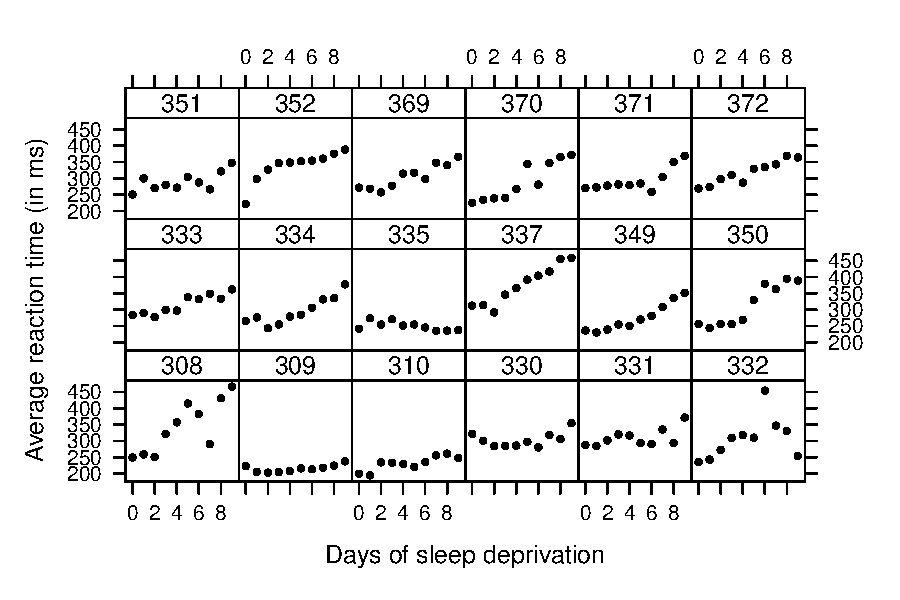
\includegraphics{figure/mtram-sleep-plot-1} 

}

\end{Schunk}
\caption{Sleep deprivation: Average reaction times to a specific task over several days 
         of sleep deprivation for $18$ subjects from
         \cite{Belenky_Wesensten_Thorne_2003}. \label{fig:sleepstudy}}
\end{figure}

The classical normal linear random-intercept/random-slope model, treating
the study participants as independent observations, is fitted by maximum
likelihood to the data using the \cmd{lmer} function from the \pkg{lme4}
add-on package \citep{pkg:lme4}:
%
\begin{Schunk}
\begin{Sinput}
R> sleep_lmer <- lmer(Reaction ~ Days + (Days | Subject), 
+                     data = sleepstudy, REML = FALSE)
\end{Sinput}
\end{Schunk}
%
The corresponding conditional model for subject $i$ reads
%
\begin{eqnarray*}
\Prob(\text{Reaction} \le \ry \mid \text{day}, i) = \Phi\left(\frac{\ry -
\alpha - \beta \text{day} - \alpha_i - \beta_i \text{day}}{\sigma}\right),
\quad (\alpha_i, \beta_i) \sim \ND_2(\nullvec, \mG(\varparm))
\end{eqnarray*}
%
with $\sigma^{-2}\mG = \mLambda(\varparm) \mLambda(\varparm)^\top$ and
%
\begin{eqnarray*}
\mLambda(\varparm) = \left( \begin{array}{cc}
    \gamma_1 & 0  \\
    \gamma_2 & \gamma_3
\end{array} \right), \quad \varparm = (\gamma_1, \gamma_2, \gamma_3)^\top.
\end{eqnarray*}

The same model, however using the alternative parameterisation and an
independent (of \pkg{lme4}, only the \cmd{update} method for Cholesky
factors is reused) gradient-based maximisation of the log-likelihood, is estimated 
in a two-step approach as
\begin{Schunk}
\begin{Sinput}
R> library("tram")
\end{Sinput}
\end{Schunk}
\begin{Schunk}
\begin{Sinput}
R> sleep_LM <- Lm(Reaction ~ Days, data = sleepstudy)
R> sleep_LMmer <- mtram(sleep_LM, ~ (Days | Subject), data = sleepstudy)
\end{Sinput}
\end{Schunk}
%
The first call to \cmd{Lm} computes the equivalent of a normal linear
regression model parameterised as a linear transformation model
\emph{ignoring} the longitudinal nature of the observations. The purpose if
to set-up the necessary model infrastructure (model matrices, inverse link
functions, etc.) and to compute reasonable starting values for the fixed
effects. The second call to \cmd{mtram} specifies the random effects
structure (here a correlated pair of random intercept for subject 
and random slope for days) and optimises the likelihood for all model
parameters $\eparm_1, \tilde{\alpha}, \tilde{\beta}$, and $\varparm$
in the model (here also looking at the conditional model for subject $i$)
%
\begin{eqnarray*}
\Prob(\text{Reaction} \le \ry \mid \text{day}, i) = \Phi\left(\eparm_1 \ry + \tilde{\alpha} - \tilde{\beta} \text{day} - \tilde{\alpha}_i - \tilde{\beta}_i \text{day}\right),
\quad (\tilde{\alpha}_i, \tilde{\beta}_i) \sim \ND_2(\nullvec, \mLambda(\varparm) \mLambda(\varparm))
\end{eqnarray*}
%
that is, all fixed and random effect parameters are 
divided by the residual standard deviation $\sigma$ (this is the
reparameterisation applied by \cmd{Lm}).
Of course, the parameter $\eparm_1$, the inverse residual standard
deviation, is ensured to be positive via an additional constraint in the
optimiser maximising the log-likelihood.
%

The log-likelihoods of the two models fitted by \cmd{lmer} and \cmd{mtram} 
are very close
\begin{Schunk}
\begin{Sinput}
R> logLik(sleep_lmer)
\end{Sinput}
\begin{Soutput}
'log Lik.' -875.9697 (df=6)
\end{Soutput}
\begin{Sinput}
R> logLik(sleep_LMmer)
\end{Sinput}
\begin{Soutput}
'log Lik.' -875.9697 (df=6)
\end{Soutput}
\end{Schunk}
Looking at the model coefficients, the two procedures lead to almost
identical inverse residual standard deviations
\begin{Schunk}
\begin{Sinput}
R> (sdinv <- 1 / summary(sleep_lmer)$sigma)
\end{Sinput}
\begin{Soutput}
[1] 0.03907485
\end{Soutput}
\begin{Sinput}
R> coef(sleep_LMmer)["Reaction"]
\end{Sinput}
\begin{Soutput}
  Reaction 
0.03907741 
\end{Soutput}
\end{Schunk}
and fixed effects (the slope can be interpreted as inverse coefficient of
variation)
\begin{Schunk}
\begin{Sinput}
R> fixef(sleep_lmer) * c(-1, 1) * sdinv
\end{Sinput}
\begin{Soutput}
(Intercept)        Days 
 -9.8236175   0.4090077 
\end{Soutput}
\begin{Sinput}
R> coef(sleep_LMmer)[c("(Intercept)", "Days")]
\end{Sinput}
\begin{Soutput}
(Intercept)        Days 
 -9.8243917   0.4089265 
\end{Soutput}
\end{Schunk}
The random-effect parameters $\varparm$ are also reasonably close
\begin{Schunk}
\begin{Sinput}
R> sleep_lmer@theta
\end{Sinput}
\begin{Soutput}
[1] 0.92919061 0.01816575 0.22264321
\end{Soutput}
\begin{Sinput}
R> coef(sleep_LMmer)[-(1:3)]
\end{Sinput}
\begin{Soutput}
    gamma1     gamma2     gamma3 
0.92901066 0.01843056 0.22280431 
\end{Soutput}
\end{Schunk}
Consequently, the variance-covariance and correlation matrices
\begin{Schunk}
\begin{Sinput}
R> sleep_LMmer$G * (1 / sdinv)^2
\end{Sinput}
\begin{Soutput}
2 x 2 sparse Matrix of class "dsCMatrix"
                      
[1,] 565.2580 11.21410
[2,]  11.2141 32.73513
\end{Soutput}
\begin{Sinput}
R> cov2cor(sleep_LMmer$G * (1 / sdinv)^2)
\end{Sinput}
\begin{Soutput}
2 x 2 sparse Matrix of class "dsCMatrix"
                          
[1,] 1.00000000 0.08243925
[2,] 0.08243925 1.00000000
\end{Soutput}
\begin{Sinput}
R> unclass(VarCorr(sleep_lmer))$Subject
\end{Sinput}
\begin{Soutput}
            (Intercept)     Days
(Intercept)   565.47697 11.05512
Days           11.05512 32.68179
attr(,"stddev")
(Intercept)        Days 
  23.779760    5.716799 
attr(,"correlation")
            (Intercept)       Days
(Intercept)  1.00000000 0.08132109
Days         0.08132109 1.00000000
\end{Soutput}
\end{Schunk}
are practically equivalent. This result indicates the correctness of the
alternative implementation of normal linear mixed-effects models in the
transformation model framework: \cmd{mtram} reuses some infrastructure from
\pkg{lme4} and \pkg{Matrix}, most importantly fast update methods for
Cholesky factors, but the likelihood and corresponding optimisation relies
on an independent implementation. So why are we doing this? Because
\cmd{mtram} is able to deal with models or likelihoods 
not available in \pkg{lme4}, for example the likelihood for
interval-censored observations.

Let's assume that the timing of the reaction times was less accurate than suggested by the
numerical representation of the results. The following code
\begin{Schunk}
\begin{Sinput}
R> library("survival")
R> sleepstudy$Reaction_I <- with(sleepstudy, Surv(Reaction - 20, Reaction + 20, 
+                                                 type = "interval2"))
R> sleepstudy$Reaction_I[1:5]
\end{Sinput}
\begin{Soutput}
[1] [229.5600, 269.5600] [238.7047, 278.7047] [230.8006, 270.8006]
[4] [301.4398, 341.4398] [336.8519, 376.8519]
\end{Soutput}
\end{Schunk}
converts the outcome to interval-censored values, where each interval has
length $40$. The above mixed model can now be estimated by maximising the
likelihood corresponding to interval-censored observations:
\begin{Schunk}
\begin{Sinput}
R> sleep_LM_I <- Lm(Reaction_I ~ Days, data = sleepstudy)
R> sleep_LMmer_I <- mtram(sleep_LM_I, ~ (Days | Subject), data = sleepstudy)
\end{Sinput}
\end{Schunk}
Of course, the log-likelihood changes (because this is a log-probability and
not a log-density of a continuous distribution) but the parameter estimates are reasonably close
\begin{Schunk}
\begin{Sinput}
R> logLik(sleep_LMmer_I)
\end{Sinput}
\begin{Soutput}
'log Lik.' -214.9675 (df=6)
\end{Soutput}
\begin{Sinput}
R> coef(sleep_LMmer_I)
\end{Sinput}
\begin{Soutput}
(Intercept)  Reaction_I        Days      gamma1      gamma2      gamma3 
-9.78770607  0.03900116  0.41633415  0.83398952  0.07584130  0.19038611 
\end{Soutput}
\begin{Sinput}
R> coef(sleep_LMmer)
\end{Sinput}
\begin{Soutput}
(Intercept)    Reaction        Days      gamma1      gamma2      gamma3 
-9.82439168  0.03907741  0.40892652  0.92901066  0.01843056  0.22280431 
\end{Soutput}
\end{Schunk}

The next question is if the normal assumption for reaction times is
appropriate. In the transformation world, this assumption is simple to
assess because we can easily (theoretically and in-silico) switch to 
the non-normal linear mixed-effects transformation model
%
\begin{eqnarray*}
\Prob(\text{Reaction} \le \ry \mid \text{day}, i) =
\Phi\left(\h(\ry) - \tilde{\beta} \text{day} - \tilde{\alpha}_i - \tilde{\beta}_i \text{day}\right),
\quad (\tilde{\alpha}_i, \tilde{\beta}_i) \sim \ND_2(\nullvec, \mLambda(\varparm) \mLambda(\varparm))
\end{eqnarray*}
%
where $\h(\ry) = \basisy(\ry)^\top \parm$ represents a monotone non-decreasing
transformation function. The function implementing such a more flexible
model in named in honor of the first paper on the analysis of
transformed responses by \cite{BoxCox_1964} but it \emph{does not} simply apply
what is known as a Box-Cox transformation. Bernstein polynomials
$\h(\ry) = \basisy(\ry)^\top \parm$ under suitable constraints 
\citep{Hothorn_Moest_Buehlmann_2017} are applied instead by
\begin{Schunk}
\begin{Sinput}
R> sleep_BC <- BoxCox(Reaction ~ Days, data = sleepstudy)
R> sleep_BCmer <- mtram(sleep_BC, ~ (Days | Subject), data = sleepstudy, 
+                       Hessian = TRUE)
R> logLik(sleep_BCmer)
\end{Sinput}
\begin{Soutput}
'log Lik.' -859.5455 (df=11)
\end{Soutput}
\end{Schunk}
%
The increase in the log-likelihood compared to the normal model is not a big
surprise.  Plotting the transformation function $\h(\ry) = \basisy(\ry)^\top \parm$ as
a function of reaction time can help to assess deviations from normality
because the latter assumption implies a linear transformation function. 
Figure~\ref{fig:sleepstudy_trafo} clearly indicates that models allowing a
certain skewness of reaction times will provide a better fit to the data.
This might also not come as a big surprise to experienced data analysts.

\begin{figure}[t]
\begin{Schunk}


{\centering 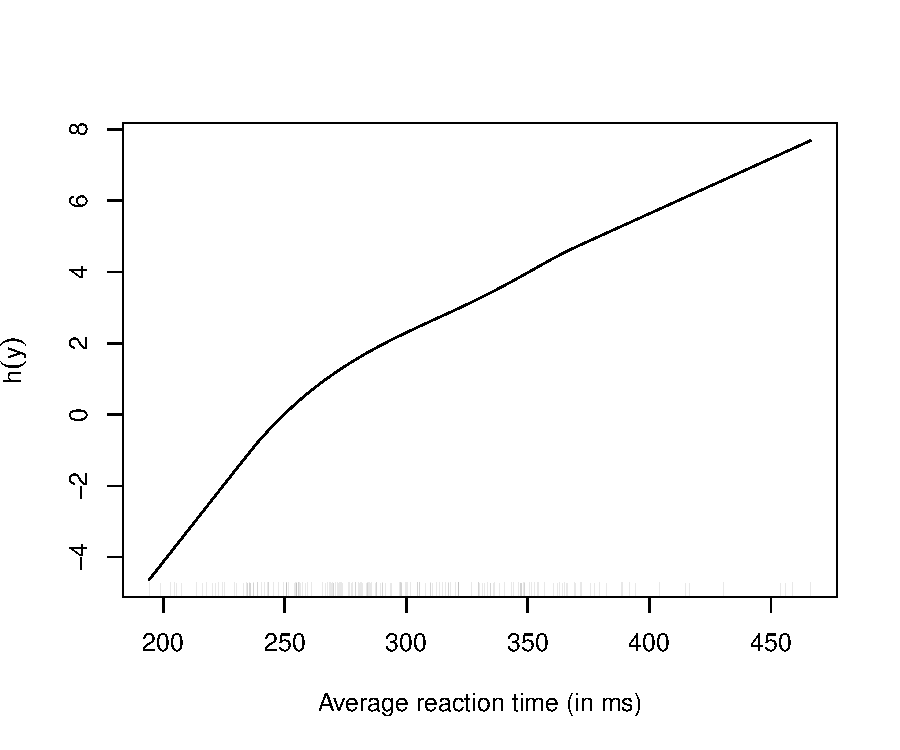
\includegraphics{figure/mtram-sleep_BoxCoxPlot-1} 

}

\end{Schunk}
\caption{Sleep deprivation: Data-driven transformation $\hat{\h}$ 
         of average reaction times to sleep deprivation. The non-linearity
         induces a non-normal marginal distribution function of reaction times.
         \label{fig:sleepstudy_trafo}}
\end{figure}

Such probit-type mixed-effects models have been studied before, mostly by merging a
Box-Cox power transformation $\h$ with a grid-search over REML estimates
\citep{Gurka_Edwards_2006}, a conditional likelihood
\citep{Hutmacher_French_2011}, or a grid-search maximising the profile
likelihood \citep{Maruo_Yamaguchi_2017}.  Recently, \THcite{Tang, Wu, and
Chen}{Tang_Wu_Chen_2018} and \THcite{Wu and Wang}{Wu_Wang_2019}
proposed a monotone spline parameterisation of $\h$ in a Bayesian context.
The model presented here was estimated by simultaneously maximising the
log-likelihood \citep{Hothorn_2019_mtram} %(\ref{fm:cll}) 
with respect to the parameters $\parm$,
$\eshiftparm$, and $\varparm$. For a linear Bernstein polynomial of order
one, the models obtained with this approach and classical maximum likelihood
estimation in normal linear mixed-effects models are equivalent (up to
reparameterisation of $\eshiftparm$).% \citep{vign:tram}.

However, what does this finding mean in terms of a direct comparison of the
model and the data?  Looking at the marginal cumulative distribution
functions of average reaction time conditional on days of sleep deprivation
in Figure~\ref{fig:sleepstudy_ecdf} one finds that the non-normal marginal
transformation models provided a better fit to the marginal empirical
cumulative distribution functions than the normal marginal models. 
Especially for short reaction times in the first week of sleep deprivation,
the orange marginal cumulative distribution is much closer to the
empirical cumulative distribution function representing the marginal
distribution of reaction times at each single day of study participation.

\begin{figure}[t]
\begin{Schunk}


{\centering 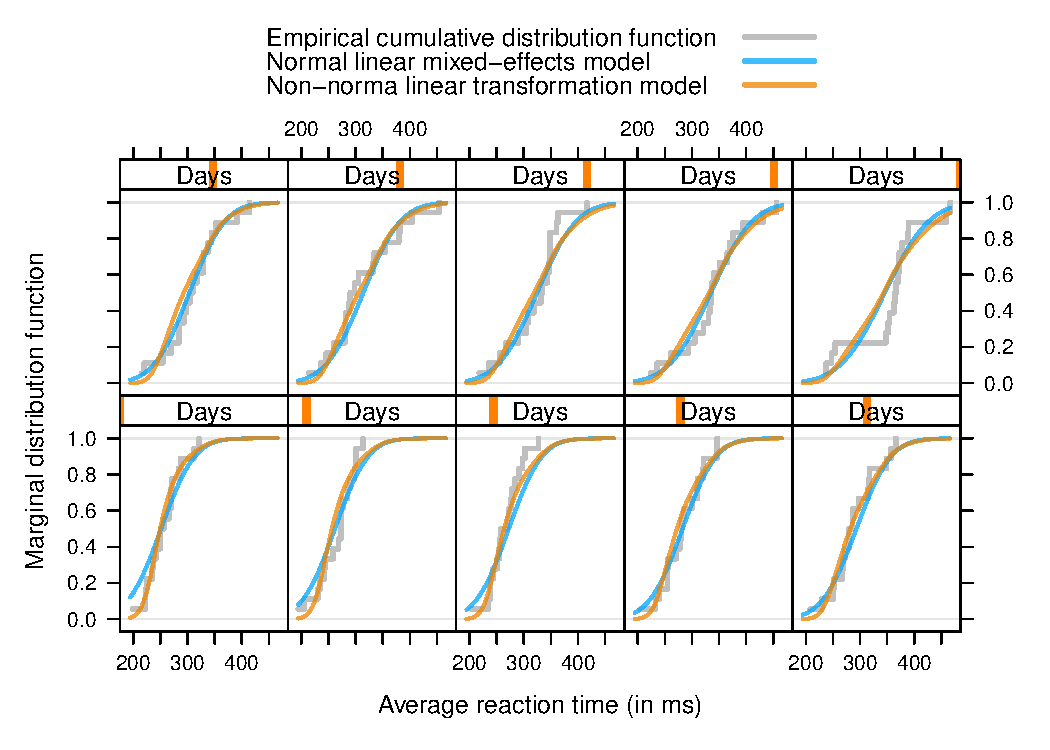
\includegraphics{figure/mtram-sleep_marginal-1} 

}

\end{Schunk}
\caption{Sleep deprivation: Marginal distribution of reaction times, separately for each day of
         study participation. The grey step-function corresponds to the
         empirical cumulative distribution function, the blue line to the
         marginal cumulative distribution of a normal linear mixed-effects model, and
         the orange line to a non-normal linear mixed-effects transformation
         model. \label{fig:sleepstudy_ecdf}}
\end{figure}

It should be noted that the small positive correlation between random intercept and random slope
observed in the normal linear mixed-effects model turned into a negative
correlation in this non-normal model 
\begin{Schunk}
\begin{Sinput}
R> cov2cor(sleep_BCmer$G)
\end{Sinput}
\begin{Soutput}
2 x 2 sparse Matrix of class "dsCMatrix"
                          
[1,]  1.0000000 -0.1946629
[2,] -0.1946629  1.0000000
\end{Soutput}
\end{Schunk}
What is the uncertainty associated with this parameter? The correlation is a
non-linear function of $\varparm$ and therefore the direct computation of
confidence intervals questionable. However, we
can extract an estimate of the covariance of the estimated model parameters
from the model and, relying on the asymptotic normality of the maximum likelihood
estimators, we can sample from the asymptotic distribution
of the variance of the random intercept $\tilde{\alpha}$, the random slope
$\tilde{\beta}$, and their correlation
\begin{Schunk}
\begin{Sinput}
R> library("mvtnorm")
R> VC <- solve(sleep_BCmer$Hessian)
R> idx <- (nrow(VC) - 2):nrow(VC)
R> Rcoef <- rmvnorm(1000, mean = coef(sleep_BCmer), sigma = VC)[,idx]
R> ret <- apply(Rcoef, 1, function(gamma) {
+      L <- matrix(c(gamma[1:2], 0, gamma[3]), nrow = 2)
+      V <- tcrossprod(L)
+      c(diag(V), cov2cor(V)[1,2])
+  })
\end{Sinput}
\end{Schunk}
The $95\%$ confidence intervals
\begin{Schunk}
\begin{Sinput}
R> ### variance random intercept
R> quantile(ret[1,], c(.025, .5, .975))
\end{Sinput}
\begin{Soutput}
     2.5%       50%     97.5% 
0.9127821 2.5713595 5.2493469 
\end{Soutput}
\begin{Sinput}
R> ### variance random slope
R> quantile(ret[2,], c(.025, .5, .975))
\end{Sinput}
\begin{Soutput}
      2.5%        50%      97.5% 
0.01890987 0.05348231 0.10594879 
\end{Soutput}
\begin{Sinput}
R> ### correlation random intercept / random slope
R> quantile(ret[3,], c(.025, .5, .975))
\end{Sinput}
\begin{Soutput}
      2.5%        50%      97.5% 
-0.6193527 -0.1883314  0.4689778 
\end{Soutput}
\end{Schunk}
indicate rather strong unobserved heterogeneity affecting the intercept and
less pronouned variability in the slope. There is only weak information
about the correlation of the two random effects contained in the data.

The downside of this approach is that, although the model is nicely
interpretable on the scale of marginal or conditional distribution
functions, the direct interpretation of the fixed effect $\tilde{\beta}$ is
not very straightforward because it corresponds to the conditional mean
\emph{after} transforming the outcome.  This interpretability issue can be
addressed by exchanging the probit link to a logit link in
Section~\ref{sec:logit}.

\section{Binary Probit Mixed-effects Models}

Here we compare different implementations of binary probit mixed models for
the notoriously difficult toe nail data \citep{backer_vroey_1998}. The
outcome was categorised to two levels (this being probably the root of all
troubles, as quasi-separation issues have been
reported by \cite{Sauter_Held_2016}).
A conditional density plot (Figure~\ref{fig:toenail}) suggests
an improvement in both treatment groups over time, however with a more rapid
advance in patients treated with terbinafine.

\begin{figure}[t]
\begin{Schunk}


{\centering 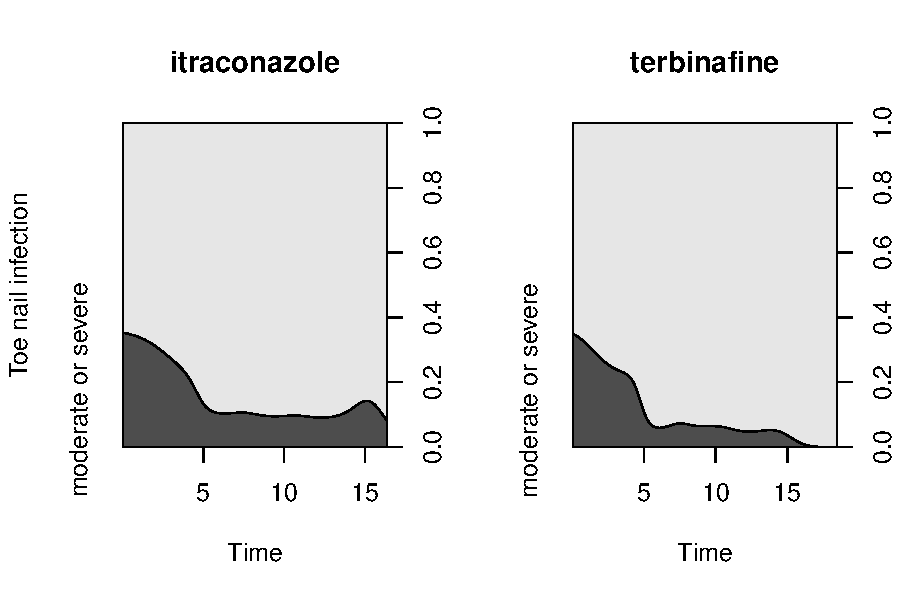
\includegraphics{figure/mtram-toenail-plot-1} 

}

\end{Schunk}
\caption{Toe nail data: Conditional density plot of two outcome classes
(none or mild vs.~moderate or severe) under two treatments.
\label{fig:toenail}}
\end{figure}

We were interested in binary probit models featuring fixed main and
interaction effects $\eshiftparm_1$, $\eshiftparm_2$, and $\eshiftparm_3$ of
treatment (itraconazole vs.~terbinafine) and time.  Subject-specific random
intercept models and models featuring correlated random intercepts and
slopes were estimated by the \code{glmer} function from package
\pkg{lme4} \citep{pkg:lme4}, by the \code{glmm} function from package
\pkg{glmmsr} \citep{ogden_2015}, and by direct maximisation of the exact
discrete log-likelihood given in Appendix B of \cite{Hothorn_2019_mtram}.
% discrete log-likelihood (\ref{fm:dll}) given in Appendix~\ref{app:cens}.

The random intercept probit model fitted by Laplace and Adaptive
Gauss-Hermite Quadrature (AGQ) approximations to the
likelihood give quite different results:
\begin{Schunk}
\begin{Sinput}
R> ### Laplace
R> toenail_glmer_RI_1 <- 
+      glmer(outcome ~ treatment * time + (1 | patientID),
+            data = toenail, family = binomial(link = "probit"), 
+            nAGQ = 1)
R> summary(toenail_glmer_RI_1)
\end{Sinput}
\begin{Soutput}
Generalized linear mixed model fit by maximum likelihood (Laplace
  Approximation) [glmerMod]
 Family: binomial  ( probit )
Formula: outcome ~ treatment * time + (1 | patientID)
   Data: toenail

     AIC      BIC   logLik deviance df.resid 
  1279.0   1306.8   -634.5   1269.0     1898 

Scaled residuals: 
   Min     1Q Median     3Q    Max 
-3.507 -0.017 -0.004  0.000 54.046 

Random effects:
 Groups    Name        Variance Std.Dev.
 patientID (Intercept) 20.68    4.548   
Number of obs: 1903, groups:  patientID, 289

Fixed effects:
                          Estimate Std. Error z value Pr(>|z|)    
(Intercept)               -3.39650    0.22091 -15.375   <2e-16 ***
treatmentterbinafine      -0.01532    0.25359  -0.060   0.9518    
time                      -0.21749    0.02256  -9.639   <2e-16 ***
treatmentterbinafine:time -0.07155    0.03425  -2.089   0.0367 *  
---
Signif. codes:  0 '***' 0.001 '**' 0.01 '*' 0.05 '.' 0.1 ' ' 1

Correlation of Fixed Effects:
            (Intr) trtmnt time  
trtmnttrbnf -0.593              
time        -0.009  0.102       
trtmnttrbn:  0.093 -0.143 -0.629
\end{Soutput}
\begin{Sinput}
R> toenail_glmer_RI_1@theta
\end{Sinput}
\begin{Soutput}
[1] 4.547891
\end{Soutput}
\begin{Sinput}
R> ### Adaptive Gaussian Quadrature
R> toenail_glmer_RI_2 <- 
+      glmer(outcome ~ treatment * time + (1 | patientID),
+            data = toenail, family = binomial(link = "probit"), 
+            nAGQ = 20)
R> summary(toenail_glmer_RI_2)
\end{Sinput}
\begin{Soutput}
Generalized linear mixed model fit by maximum likelihood (Adaptive
  Gauss-Hermite Quadrature, nAGQ = 20) [glmerMod]
 Family: binomial  ( probit )
Formula: outcome ~ treatment * time + (1 | patientID)
   Data: toenail

     AIC      BIC   logLik deviance df.resid 
  1277.8   1305.6   -633.9   1267.8     1898 

Scaled residuals: 
   Min     1Q Median     3Q    Max 
-2.847 -0.189 -0.078 -0.001 33.997 

Random effects:
 Groups    Name        Variance Std.Dev.
 patientID (Intercept) 4.485    2.118   
Number of obs: 1903, groups:  patientID, 289

Fixed effects:
                          Estimate Std. Error z value Pr(>|z|)    
(Intercept)               -0.93061    0.23176  -4.015 5.93e-05 ***
treatmentterbinafine      -0.07609    0.30921  -0.246   0.8056    
time                      -0.19074    0.02059  -9.263  < 2e-16 ***
treatmentterbinafine:time -0.06419    0.03099  -2.071   0.0383 *  
---
Signif. codes:  0 '***' 0.001 '**' 0.01 '*' 0.05 '.' 0.1 ' ' 1

Correlation of Fixed Effects:
            (Intr) trtmnt time  
trtmnttrbnf -0.655              
time        -0.186  0.212       
trtmnttrbn:  0.193 -0.287 -0.611
\end{Soutput}
\begin{Sinput}
R> toenail_glmer_RI_2@theta
\end{Sinput}
\begin{Soutput}
[1] 2.117846
\end{Soutput}
\end{Schunk}

The sequential reduction (SR) algorithm \citep{ogden_2015} gives results close to
AGQ
\begin{Schunk}
\begin{Sinput}
R> library("glmmsr")
\end{Sinput}
\end{Schunk}
\begin{Schunk}
\begin{Sinput}
R> toenail_glmm_RI_3 <- 
+      glmm(outcome ~ treatment * time + (1 | patientID),
+           data = toenail, family = binomial(link = "probit"), 
+           method = "SR", control = list(nSL = 3))
\end{Sinput}
\begin{Soutput}
Fitting the model................. done.
\end{Soutput}
\begin{Sinput}
R> summary(toenail_glmm_RI_3)
\end{Sinput}
\begin{Soutput}
Generalized linear mixed model fit by maximum likelihood [glmmFit] 
Likelihood approximation: Sequential reduction at level 3 
 
Family: binomial ( probit ) 
Formula: outcome ~ treatment * time + (1 | patientID)

Random effects:
 Groups    Name        Estimate Std.Error
 patientID (Intercept) 2.119    0.1954   
Number of obs: 1903, groups: patientID, 289; 

Fixed effects: 
                          Estimate Std. Error z value  Pr(>|z|)
(Intercept)               -0.93105    0.23217  4.0102 6.066e-05
treatmentterbinafine      -0.07618    0.30945  0.2462 8.055e-01
time                      -0.19076    0.02060  9.2618 2.010e-20
treatmentterbinafine:time -0.06420    0.03099  2.0713 3.834e-02
\end{Soutput}
\end{Schunk}

Because of the probit link, this binary generalised linear model is
equivalent to a linear transformation model and we can thus use the exact
likelihood implemented for the latter model in \cmd{mtram} for parameter
estimation (it is still a bit nasty to set-up a constant transformation function
$\h(\ry) = \alpha$, we plan to add a more convenient interface later)
\begin{Schunk}
\begin{Sinput}
R> m <- ctm(as.basis(~ outcome, data = toenail), 
+           shifting = ~ treatment * time, 
+           data = toenail, todistr = "Normal")
R> toenail_probit <- mlt(m, data = toenail, 
+                        fixed = c("outcomemoderate or severe" = 0))
R> toenail_mtram_RI <- 
+      mtram(toenail_probit, ~ (1 | patientID), 
+            data = toenail, Hessian = TRUE)
R> coef(toenail_mtram_RI)
\end{Sinput}
\begin{Soutput}
              (Intercept)      treatmentterbinafine 
               0.92947317                0.07699415 
                     time treatmentterbinafine:time 
               0.19056726                0.06355500 
                   gamma1 
               2.11448400 
\end{Soutput}
\end{Schunk}
For this random intercept model, the exact likelihood is defined as a
one-dimensional integral over the unit interval.  We use sparse grids
\citep{Heiss_Winschel_2008, pkg:SparseGrid} to approximate this integral. 
The integrand is defined by products of normal probabilities, which are
approximated as described by \cite{Matic_Radoicic_2018}.  It is important to
note that this likelihood can be computed as accurately as necessary whereas
Laplace, AGQ, and SR are approximations of limited accuracy. 

The results are very close to SR and AGQ, indicating a very good quality of
the AGQ and SR approximations. We can also compare the corresponding covariances
\begin{Schunk}
\begin{Sinput}
R> vcov(toenail_glmer_RI_2)
\end{Sinput}
\begin{Soutput}
4 x 4 Matrix of class "dpoMatrix"
                            (Intercept) treatmentterbinafine          time
(Intercept)                0.0537124461         -0.046953347 -0.0008877032
treatmentterbinafine      -0.0469533473          0.095609207  0.0013522295
time                      -0.0008877032          0.001352229  0.0004239967
treatmentterbinafine:time  0.0013871385         -0.002754664 -0.0003896724
                          treatmentterbinafine:time
(Intercept)                            0.0013871385
treatmentterbinafine                  -0.0027546636
time                                  -0.0003896724
treatmentterbinafine:time              0.0009603449
\end{Soutput}
\begin{Sinput}
R> solve(toenail_mtram_RI$Hessian)[1:4, 1:4]
\end{Sinput}
\begin{Soutput}
              [,1]         [,2]          [,3]          [,4]
[1,]  0.0535097423 -0.046828787 -0.0008863008  0.0013728404
[2,] -0.0468287869  0.095401755  0.0013454564 -0.0027201727
[3,] -0.0008863008  0.001345456  0.0004223674 -0.0003889295
[4,]  0.0013728404 -0.002720173 -0.0003889295  0.0009479493
\end{Soutput}
\end{Schunk}
%We can compare the in-sample log-likelihood (as defined by the
%transformation model) for parameter estimates obtained from 
%the different procedures
%<<mtram-toenail_RI_mlt_glmmsr>>=
%### logLik of transformation model for glmer (Laplace) parameters
%logLik(toenail_mtram_RI, c(-fixef(toenail_glmer_RI_1), 
%                            toenail_glmer_RI_1@theta))
%### logLik of transformation model for glmer (AGQ) parameters
%logLik(toenail_mtram_RI, c(-fixef(toenail_glmer_RI_2), 
%                            toenail_glmer_RI_2@theta))
%### logLik of transformation model for glmmsr (SR) parameters
%logLik(toenail_mtram_RI, parm = c(-toenail_glmm_RI_3$estim[-1], 
%                                   toenail_glmm_RI_3$estim[1]))
%### logLik of transformation model
%logLik(toenail_mtram_RI)
%@
%Except for the Laplace approximation, the in-sample log-likelihoods
%coincide.

Things get a bit less straightforward when a random slope is added to the
model. The two implementations of the Laplace approximation in packages
\pkg{lme4}
\begin{Schunk}
\begin{Sinput}
R> toenail_glmer_RS <- 
+      glmer(outcome ~ treatment * time + (1 + time | patientID),
+            data = toenail, family = binomial(link = "probit"))
R> summary(toenail_glmer_RS)
\end{Sinput}
\begin{Soutput}
Generalized linear mixed model fit by maximum likelihood (Laplace
  Approximation) [glmerMod]
 Family: binomial  ( probit )
Formula: outcome ~ treatment * time + (1 + time | patientID)
   Data: toenail

     AIC      BIC   logLik deviance df.resid 
   985.8   1024.7   -485.9    971.8     1896 

Scaled residuals: 
     Min       1Q   Median       3Q      Max 
-1.85421 -0.00210 -0.00037  0.00000  2.35828 

Random effects:
 Groups    Name        Variance Std.Dev. Corr 
 patientID (Intercept) 118.433  10.883        
           time          3.305   1.818   -0.90
Number of obs: 1903, groups:  patientID, 289

Fixed effects:
                          Estimate Std. Error z value Pr(>|z|)    
(Intercept)               -4.30120    0.26361 -16.316   <2e-16 ***
treatmentterbinafine       0.05419    0.34652   0.156   0.8757    
time                      -0.06792    0.07847  -0.866   0.3867    
treatmentterbinafine:time -0.23478    0.13885  -1.691   0.0909 .  
---
Signif. codes:  0 '***' 0.001 '**' 0.01 '*' 0.05 '.' 0.1 ' ' 1

Correlation of Fixed Effects:
            (Intr) trtmnt time  
trtmnttrbnf -0.662              
time        -0.453  0.342       
trtmnttrbn:  0.270 -0.438 -0.335
\end{Soutput}
\begin{Sinput}
R> toenail_glmer_RS@theta
\end{Sinput}
\begin{Soutput}
[1] 10.8826790 -1.6359589  0.7930842
\end{Soutput}
\end{Schunk}

and \pkg{glmmsr}
\begin{Schunk}
\begin{Sinput}
R> toenail_glmm_RS_1 <- 
+      glmm(outcome ~ treatment * time + (1 + time | patientID),
+           data = toenail, family = binomial(link = "probit"), 
+           method = "Laplace")
\end{Sinput}
\begin{Soutput}
Fitting the model... done.
\end{Soutput}
\begin{Sinput}
R> toenail_glmm_RS_1$estim[1:3]
\end{Sinput}
\begin{Soutput}
[1]  4.9992120 -0.5708117  0.4234373
\end{Soutput}
\begin{Sinput}
R> toenail_glmm_RS_1$estim[-(1:3)]
\end{Sinput}
\begin{Soutput}
[1] -3.492610943  0.009300918 -0.065461048 -0.133223336
\end{Soutput}
\end{Schunk}
do not quite agree. Note that the standard deviation of the random intercept
is twice as large in the \cmd{glmer} output.

The optimisation of the exact discrete likelihood in the transformation
framework gives
\begin{Schunk}
\begin{Sinput}
R> toenail_mtram_RS <- 
+      mtram(toenail_probit, ~ (1 + time | patientID), 
+            data = toenail)
R> logLik(toenail_mtram_RS)
\end{Sinput}
\begin{Soutput}
'log Lik.' -545.1164 (df=7)
\end{Soutput}
\begin{Sinput}
R> coef(toenail_mtram_RS)
\end{Sinput}
\begin{Soutput}
              (Intercept)      treatmentterbinafine 
                1.5765323                -0.2666843 
                     time treatmentterbinafine:time 
                0.5323919                 0.1842506 
                   gamma1                    gamma2 
                5.2172371                -0.3723897 
                   gamma3 
                0.5285640 
\end{Soutput}
\end{Schunk}
The variance parameters are not too far off the results reported by
\cmd{glmm}, but the fixed effects differ quite a bit. 
%Again, we can
%compare the in-sample log-likelihoods:
%<<mtram-toenail_RS_mlt_glmmsr>>=
%### logLik of transformation model for glmer (Laplace) parameters
%logLik(toenail_mtram_RS, c(-fixef(toenail_glmer_RS), 
%                            toenail_glmer_RS@theta))
%### logLik of transformation model for glmmsr (Laplace) parameters
%logLik(toenail_mtram_RS, parm = c(-toenail_glmm_RS_1$estim[-(1:3)], 
%                                   toenail_glmm_RS_1$estim[1:3]))
%### logLik of transformation model
%logLik(toenail_mtram_RS)
%@

At least in biostatistics, the probit model is less popular than the logit
model owing to the better interpretability of the fixed effects as
conditional log-odds ratios in the latter. Using a logit link, we can use
the transformation approach to compute marginally interpretable
time-dependent log-odds ratios from random intercept transformation logit
models:% \citep[\code{standardise = TRUE} computes model (M2) instead of the
%default (M1), see][]{Hothorn_2019_mtram}:
\begin{Schunk}
\begin{Sinput}
R> m <- ctm(as.basis(~ outcome, data = toenail), 
+           shifting = ~ treatment * time, 
+           data = toenail, todistr = "Logistic")
R> toenail_logit <- mlt(m, data = toenail, 
+                       fixed = c("outcomemoderate or severe" = 0))
R> toenail_mtram_logit <- mtram(toenail_logit, ~ (1 | patientID), 
+                               data = toenail, Hessian = TRUE)
\end{Sinput}
\end{Schunk}
It is important to note that this model is \emph{not} a logistic 
mixed-effects model and thus we can't expect to obtain identical 
results from \cmd{glmer} as it was (partially) the case for the probit
model.

From the model, we can compute marginally interpretable 
probabilities and odds ratios over time
\begin{Schunk}
\begin{Sinput}
R> tmp <- toenail_logit
R> cf <- coef(tmp)
R> cf <- cf[names(cf) != "outcomemoderate or severe"]
R> sdrf <- rev(coef(toenail_mtram_logit))[1]
R> cf <- coef(toenail_mtram_logit)[names(cf)] / sqrt(sdrf^2 + 1)
R> cf <- c(cf[1], "outcomemoderate or severe" = 0, cf[-1])
R> coef(tmp) <- cf
R> time <- 0:180/10
R> treatment <- sort(unique(toenail$treatment))
R> nd <- expand.grid(time = time, treatment = treatment)
R> nd$prob_logit <- predict(tmp, newdata = nd, type = "distribution")[1,]
R> nd$odds <- exp(predict(tmp, newdata = nd, type = "trafo")[1,])
\end{Sinput}
\end{Schunk}

We can also sample from the distribution of the maximum likelihood
estimators to obtain an idea about the uncertainty
(Figure~\ref{fig:toenailOR}).

\begin{figure}[t]
\begin{Schunk}


{\centering 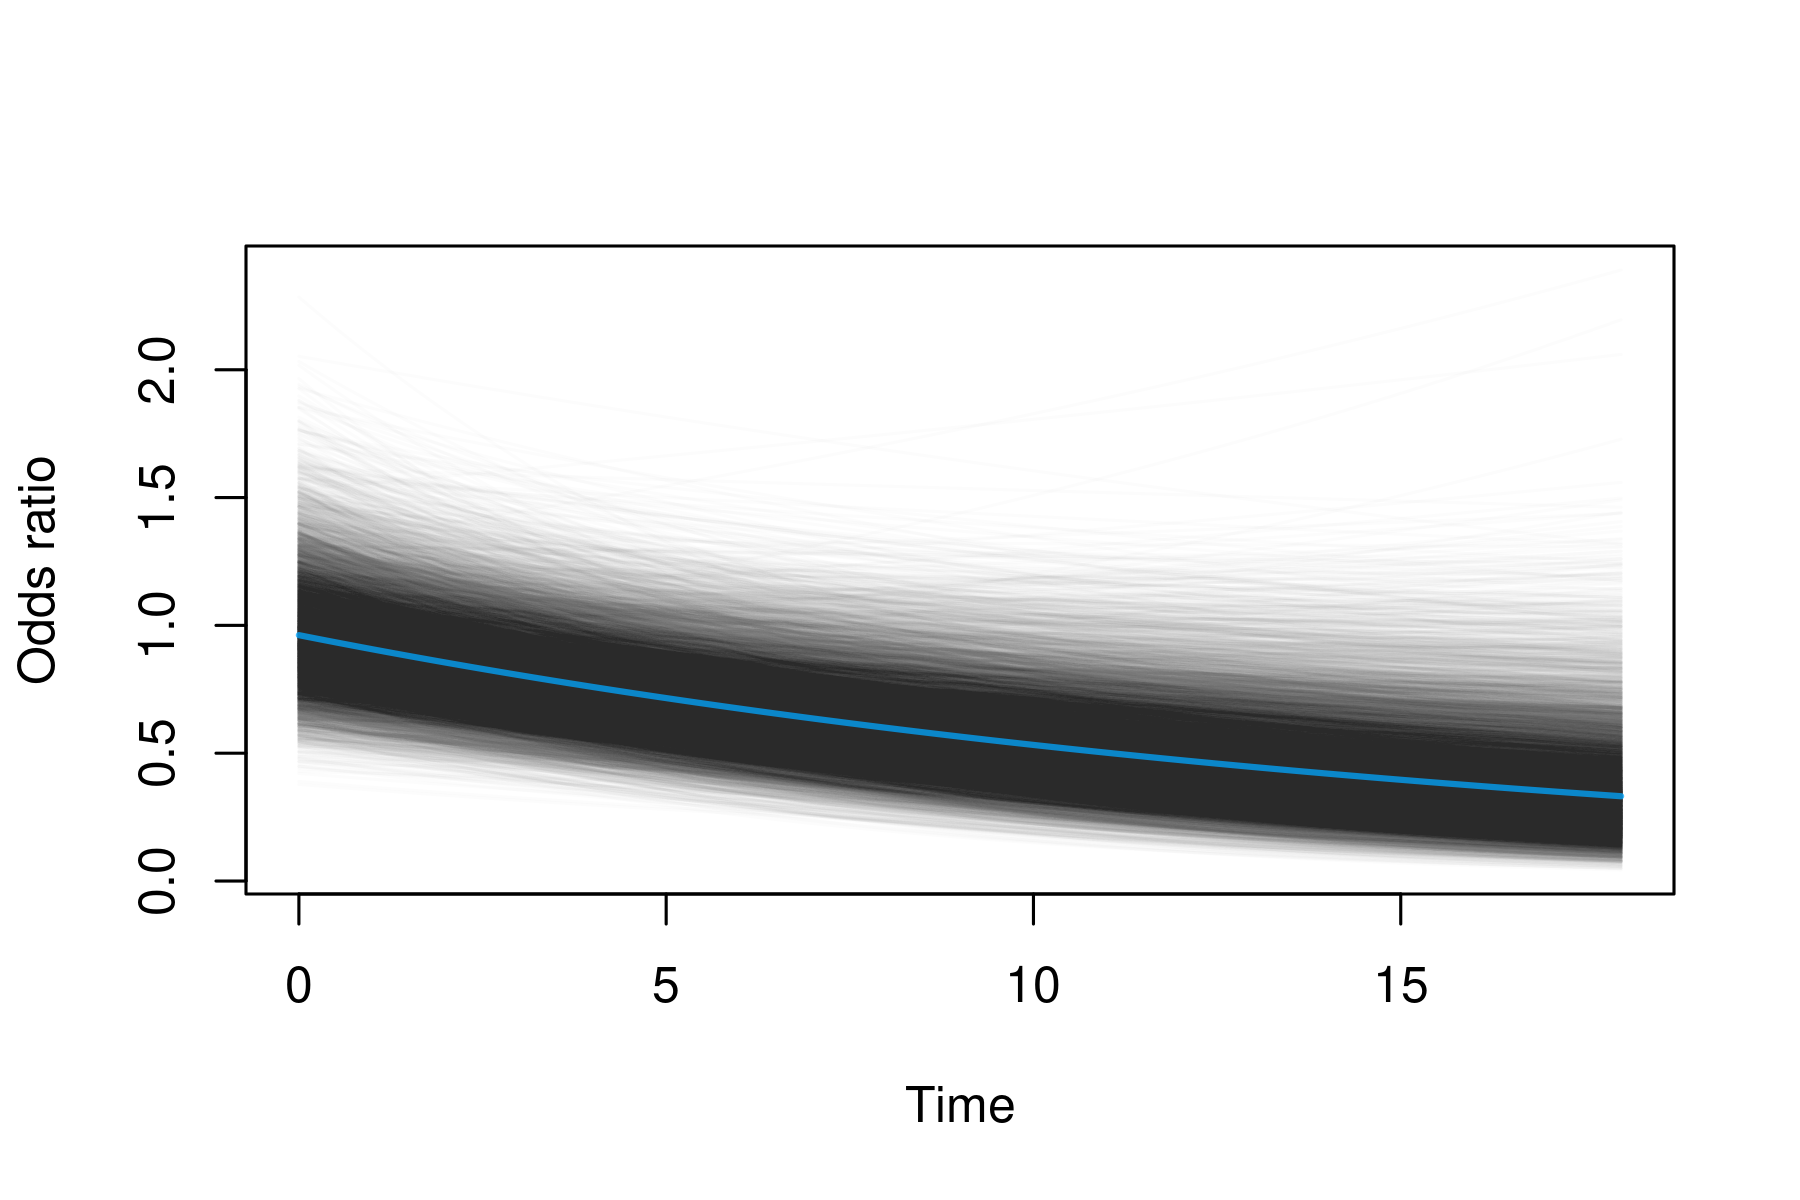
\includegraphics{figure/mtram-toenail_OR_2-1} 

}

\end{Schunk}
\caption{Toe nail data: Marginal odds ratio over time (from a logistic
  random intercept model). The blue line represents the maximum likelihood
  estimator, the grey lines are samples from the corresponding distribution.
  \label{fig:toenailOR}}
\end{figure}

From the logit and probit models, we can also obtain
marginally interpretable probabilities as (probit)
\begin{Schunk}
\begin{Sinput}
R> tmp <- toenail_logit
R> cf <- coef(tmp)
R> cf <- cf[names(cf) != "outcomemoderate or severe"]
R> sdrf <- rev(coef(toenail_mtram_logit))[1]
R> cf <- coef(toenail_mtram_logit)[names(cf)] 
R> cf <- c(cf[1], "outcomemoderate or severe" = 0, cf[-1])
R> coef(tmp) <- cf
R> pr <- predict(tmp, newdata = nd, type = "distribution")[1,]
R> nd$prob_logit <- pnorm(qnorm(pr) / sdrf)
\end{Sinput}
\end{Schunk}
and (logit)
\begin{Schunk}
\begin{Sinput}
R> tmp <- toenail_probit
R> cf <- coef(tmp)
R> cf <- cf[names(cf) != "outcomemoderate or severe"]
R> sdrf <- rev(coef(toenail_mtram_RI))[1]
R> cf <- coef(toenail_mtram_RI)[names(cf)] / sqrt(sdrf^2 + 1)
R> cf <- c(cf[1], "outcomemoderate or severe" = 0, cf[-1])
R> coef(tmp) <- cf
R> nd$prob_probit <- predict(tmp, newdata = nd, type = "distribution")[1,]
\end{Sinput}
\end{Schunk}
The marginal time-dependent probabilities obtained from all three models are
very similar as shown in Figure~\ref{fig:toenailprob}.

\begin{figure}[t]
\begin{Schunk}


{\centering 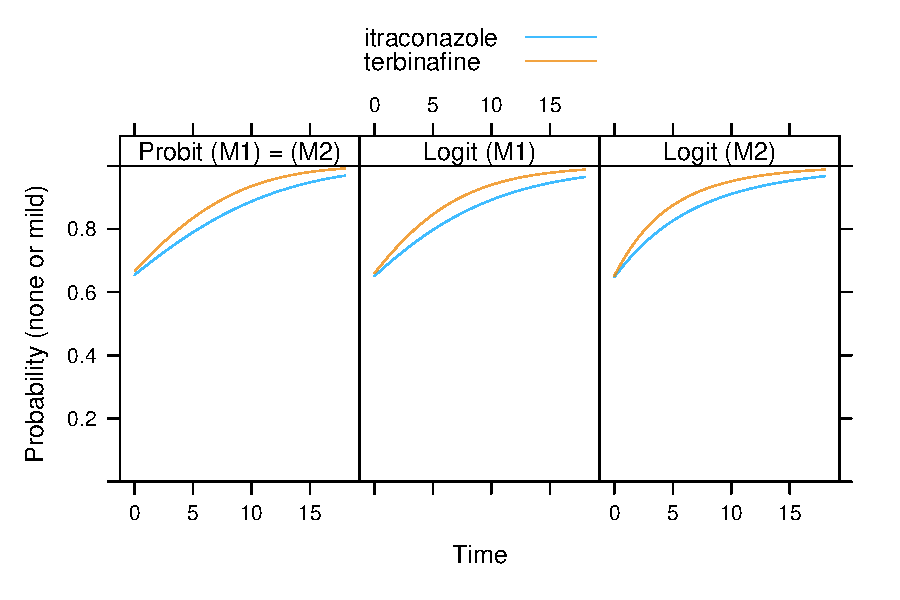
\includegraphics{figure/mtram-toenail_probplot-1} 

}

\end{Schunk}
\caption{Toe nail data: Comparison of marginal probabilities obtained from
         a probit linear mixed-effects model and 
         a logistic transformation
         model with marginal log-odds ratio treatment effect.
         % two logistic transformation
         % models (M2: with or M1: without marginal log-odds ratio treatment
         % effect). 
         \label{fig:toenailprob}}
\end{figure}

The estimated model parameters, along with the discrete log-likelihood
\citep[Equation~7 in][]{Hothorn_2019_mtram} evaluated at these parameters, are given in
Table~\ref{tab:toenail}.  For the random intercept models, AGQ, SR, and the
discrete log-likelihood give the same results, the Laplace approximation
seemed to fail.  It was not possible to apply the AGQ and SR approaches to
the random intercept / random slope model.  The two implementations of the
Laplace approximation in packages \pkg{lme4} and \pkg{glmmsr} differed
quite a bit.  The log-likelihood obtained by direct maximisation of
(7) resulted in the best fitting model with
the least extreme parameter estimates.  
Computing times for all procedures were comparable.

\begin{table}
\begin{center}
%%%% coefs, logLiks, and timings in table


\begin{tabular}{lrrrr|rrr} \\ \hline
& \multicolumn{4}{c|}{RI} & \multicolumn{3}{c}{RI + RS} \\
& \texttt{glmer} & \texttt{glmer} & \texttt{glmm} &  & \texttt{glmer} & \texttt{glmm} & \\
& L               & AGQ             & SR & (7) & L & L & (7) \\ \hline
$\alpha$ & -3.40 & -0.93 & -0.93 & -0.93 & -4.30 & -3.49 & -1.58
\\
$\eshiftparm_1$ & -0.02 & -0.08 & -0.08 & -0.08 &  0.05 &  0.01 &  0.27
\\
$\eshiftparm_2$ & -0.22 & -0.19 & -0.19 & -0.19 & -0.07 & -0.07 & -0.53
\\
$\eshiftparm_3$ & -0.07 & -0.06 & -0.06 & -0.06 & -0.23 & -0.13 & -0.18
\\
$\gamma_1$ &  4.55 &  2.12 &  2.12 &  2.11 & 10.88 &  5.00 &  5.22
\\
$\gamma_2$ &  0.00 &  0.00 &  0.00 &  0.00 & -1.64 & -0.57 & -0.37
\\
$\gamma_3$ &  0.00 &  0.00 &  0.00 &  0.00 &  0.79 &  0.42 &  0.53
\\
\hline
LogLik & -671.27&-633.96&-633.96&-633.96&-628.12&-575.56&-545.12 \\ 
Time (sec)   &  3.16& 1.79&21.14& 2.32&10.06& 5.31&11.83 \\ \hline
\end{tabular}

\caption{Toe nail data. Binary probit models featuring fixed intercepts
$\alpha$, treatment effects $\eshiftparm_1$, time effects $\eshiftparm_2$,
and time-treatment interactions $\eshiftparm_3$ are compared.
Random intercept (RI) and
random intercept/random slope (RI + RS) models were estimated by the Laplace (L),
Adaptive Gauss-Hermite Quadrature (AGQ), an Sequential
Reduction (SR) approximations to the likelihood (implemented in packages
\pkg{lme4} and \pkg{glmmsr}). In addition, the exact discrete
log-likelihood (7) was used for model fitting and evaluation (the
in-sample log-likelihood (7) for all models and timings
of all procedures are given in the last two lines).
\label{tab:toenail}
}
\end{center}
\end{table}


\section{Proportional Odds Models for Bounded Responses} \label{sec:logit}

\cite{manuguerra_heller_2010} proposed a mixed-effects model for bounded
responses  whose fixed effects can be interpreted as log-odds ratios. 
We fit a transformation model to data from
a randomised controlled trial on chronic neck pain treatment
\citep{chow_heller_2006}. The data are visualised in
Figure~\ref{fig:neck_pain}. Subjective neck pain levels were assessed on a 
visual analog scale, that is, on a bounded interval.

\begin{figure}[t]
\begin{Schunk}


{\centering 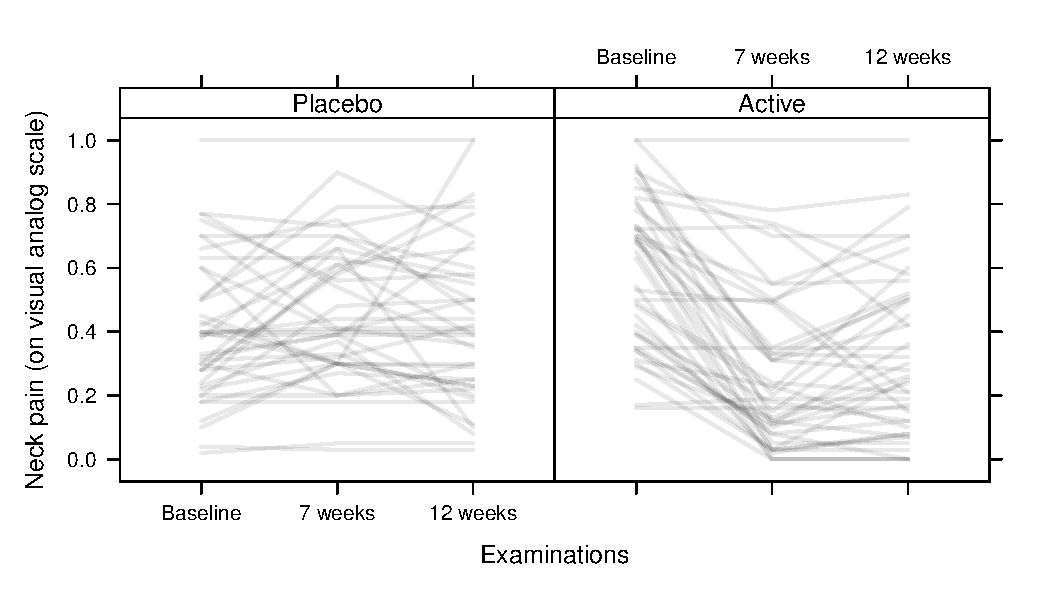
\includegraphics{figure/mtram-neck_plot-1} 

}

\end{Schunk}
\caption{Neck pain: Trajectories of neck pain assessed on a visual analog
         scale with and without low-level laser therapy.
         \label{fig:neck_pain}}
\end{figure}

\cite{manuguerra_heller_2010} suggested the conditional model
\begin{eqnarray*}
& & \logit(\Prob(\text{pain} \le \ry \mid \text{treatment}, \text{time}, i)) =
\\
& &  \quad \h(\ry) + \eshiftparm_\text{Active} + \eshiftparm_\text{7 weeks} + 
  \eshiftparm_\text{12 weeks} + \eshiftparm_\text{7 weeks, Active} + 
  \eshiftparm_\text{12 weeks, Active} + \alpha_i
\end{eqnarray*}
with random intercepts $\tilde{\alpha}_i$ such that the odds at baseline, for example, are given by
\begin{eqnarray*}
\frac{\Prob(\text{pain} \le \ry \mid \text{Active}, \text{baseline}, i)}
     {\Prob(\text{pain} > \ry \mid \text{Active}, \text{baseline}, i)} = 
\exp(\eshiftparm_\text{Active}) 
\frac{\Prob(\text{pain} \le \ry \mid \text{Placebo}, \text{baseline}, i)}
     {\Prob(\text{pain} > \ry \mid \text{Placebo}, \text{baseline}, i)}
\end{eqnarray*}

\begin{Schunk}
\begin{Sinput}
R> library("ordinalCont")
\end{Sinput}
\end{Schunk}
\begin{Schunk}
\begin{Sinput}
R> neck_ocm <- ocm(vas ~ laser * time + (1 | id), data = pain_df, 
+                  scale = c(0, 1))
\end{Sinput}
\end{Schunk}
The results
\begin{Schunk}
\begin{Sinput}
R> summary(neck_ocm)
\end{Sinput}
\begin{Soutput}
Call:
ocm(formula = vas ~ laser * time + (1 | id), data = pain_df, 
    scale = c(0, 1))

Random effects:
         Name Variance Std.Dev.
 Intercept|id    5.755    2.399

Coefficients:
                         Estimate   StdErr t.value   p.value    
laserActive              -2.07922  0.65055 -3.1961  0.001918 ** 
time7 weeks              -0.60366  0.35744 -1.6889  0.094689 .  
time12 weeks             -0.23804  0.36365 -0.6546  0.514395    
laserActive:time7 weeks   4.40817  0.56073  7.8615 7.604e-12 ***
laserActive:time12 weeks  3.38593  0.53925  6.2790 1.159e-08 ***
---
Signif. codes:  0 '***' 0.001 '**' 0.01 '*' 0.05 '.' 0.1 ' ' 1
\end{Soutput}
\end{Schunk}
suggest that there is a difference at baseline; the pain distribution of 
subjects in the placebo group on the odds scale is only 
$12.5\%$ of the odds in the active 
group for any cut-off $\ry$:
\begin{Schunk}
\begin{Sinput}
R> exp(cbind(coef(neck_ocm)[2:6], confint(neck_ocm)[2:6,]))
\end{Sinput}
\begin{Soutput}
                                          2.5 %      97.5 %
laserActive               0.1250278  0.03493482   0.4474608
time7 weeks               0.5468040  0.27137954   1.1017581
time12 weeks              0.7881704  0.38643700   1.6075391
laserActive:time7 weeks  82.1194073 27.36208405 246.4577275
laserActive:time12 weeks 29.5454666 10.26785879  85.0162253
\end{Soutput}
\end{Schunk}
In contrast, there seems to be a very large treatment effect (at week 7, the
odds in the placebo group is $0.55$ times
larger than in the active group. This levels off after 12 weeks, but the
effect is still significant at the $5\%$ level.

For comparison, we can fit a conditional mixed-effects transformation model with a different
parametrisation of the transformation function $\h$ using a Laplace
approximation of the likelihood \citep{Tamasi_Crowther_Puhan_2022}:
\begin{Schunk}
\begin{Sinput}
R> library("tramME")
R> neck_ColrME <- ColrME(vas ~ laser * time + (1 | id), data = pain_df, 
+                        bounds = c(0, 1), support = c(0, 1))
\end{Sinput}
\end{Schunk}
and coefficients
\begin{Schunk}
\begin{Sinput}
R> exp(coef(neck_ColrME))
\end{Sinput}
\begin{Soutput}
             laserActive              time7 weeks             time12 weeks 
               0.1040042                0.5184702                0.7806349 
 laserActive:time7 weeks laserActive:time12 weeks 
             130.6994999               41.9850813 
\end{Soutput}
\end{Schunk}
The model is the same as \code{neck\_ocm}, but the parameter estimates for
log-odds ratios differ quite substantially due to an alternative
parameterisation of $\h$ and due to different estimation procedures being
applied.

Our marginally interpretable transformation model with the same
transformation function as the model \code{neck\_ColrME} but with a completely 
different model formulation and optimisation procedure for maximising the log-likelihood, 
can be estimated by
\begin{Schunk}
\begin{Sinput}
R> neck_Colr <- Colr(vas ~ laser * time, data = pain_df, 
+                    bounds = c(0, 1), support = c(0, 1),
+                    extrapolate = TRUE)
R> neck_Colrmer <- mtram(neck_Colr, ~ (1 | id), data = pain_df, 
+                        Hessian = TRUE)
\end{Sinput}
\end{Schunk}
Based on this model, it is possible to derive the marginal 
distribution functions in the two groups, see Figure~\ref{fig:distr_pain}.

\begin{figure}[t]
\begin{Schunk}


{\centering 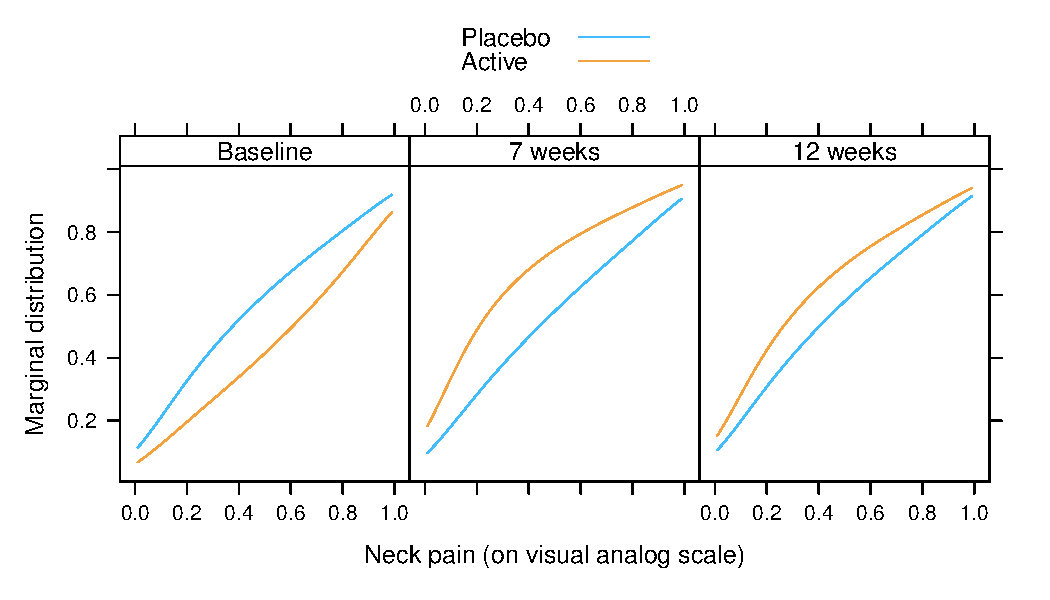
\includegraphics{figure/mtram-neck_Colr_distr-1} 

}

\end{Schunk}
\caption{Neck pain: Marginal distribution functions of chronic neck pain
         evaluated at three different time points under placebo or active
         low-level laser therapy. \label{fig:distr_pain}}
\end{figure}
We sample from the joint normal distribution of the maximum likelihood estimators
$\hat{\eparm}_1, \dots, \hat{\eparm}_7$, $\hat{\eshiftparm}_\text{Active},
\hat{\eshiftparm}_\text{7 weeks}, \hat{\eshiftparm}_\text{12 weeks},
\hat{\eshiftparm}_\text{7 weeks, Active},
\hat{\eshiftparm}_\text{12 weeks, Active}, \hat{\alpha}_i$
and compute confidence intervals for the marginal treatment
effect after 7 and 12 weeks
\begin{Schunk}
\begin{Sinput}
R> S <- solve(neck_Colrmer$Hessian)
R> rbeta <- rmvnorm(10000, mean = coef(neck_Colrmer), sigma = S)
R> s <- rbeta[, ncol(rbeta)]
R> rbeta <- rbeta[,-ncol(rbeta)] / sqrt(s^2 + 1)
R> t(apply(rbeta[, 8:12], 2, function(x) {
+    quantile(exp(x),prob = c(.025, .5, .975))}))
\end{Sinput}
\begin{Soutput}
                              2.5%        50%      97.5%
laserActive              0.1155597  0.2442656  0.5116651
time7 weeks              0.4440986  0.6910827  1.0546846
time12 weeks             0.5493419  0.8541083  1.3186687
laserActive:time7 weeks  7.8967729 15.6946073 33.8065001
laserActive:time12 weeks 4.3462218  8.5281613 17.5073242
\end{Soutput}
\end{Schunk}

Because the model \code{neck_Colrmer} has a marginal interpretation, we can
derive the marginal probabilistic index and corresponding confidence intervals 
for the three time points as follows. In this case, the marginal probabilistic
index obtained from model \code{neck\_Colrmer} is the probability that,
for a randomly selected patient in the treatment group, the neck pain score at 
time $t$ is higher than the score for a subject in the placebo group randomly 
selected at the same time point. 

There are two possible ways to compute the marginal probabilistic index.
First, we consider the standardised version of the marginal treatment effects,
that is:
\begin{Schunk}
\begin{Sinput}
R> beta <- coef(neck_Colrmer)[8:12]
R> alpha <- coef(neck_Colrmer)[13]
R> (std_beta <- cbind(beta / sqrt(1 + alpha^2)))
\end{Sinput}
\begin{Soutput}
                               [,1]
laserActive              -1.4103130
time7 weeks              -0.3700945
time12 weeks             -0.1603065
laserActive:time7 weeks   2.7556704
laserActive:time12 weeks  2.1411043
\end{Soutput}
\end{Schunk}
Then we compute the marginal treatment effect for weeks $0, 7, 12$ by multiplying
the shift vector with the following contrast matrix
\begin{Schunk}
\begin{Sinput}
R> ctr_mat <- matrix(c(1, 0, 0, 0, 0,
+                      1, 0, 0, 1, 0,
+                      1, 0, 0, 0, 1), nrow = 3, byrow = TRUE)
R> ctr_mat %*% std_beta
\end{Sinput}
\begin{Soutput}
           [,1]
[1,] -1.4103130
[2,]  1.3453573
[3,]  0.7307912
\end{Soutput}
\end{Schunk}
We simulate from the asymptotic distribution of the parameters to obtain an
empirical 95\% confidence interval and pass it to the \code{PI} function by
specifying the correct link function
\begin{Schunk}
\begin{Sinput}
R> (ci_emp <- t(apply(ctr_mat %*% t(rbeta[, 8:12]), 1, function(x) {
+    quantile(x, prob = c(.025, .5, .975))})))
\end{Sinput}
\begin{Soutput}
            2.5%        50%      97.5%
[1,] -2.15796821 -1.4094990 -0.6700849
[2,]  0.59267791  1.3457813  2.1487890
[3,] -0.02692987  0.7356106  1.5289845
\end{Soutput}
\begin{Sinput}
R> PI(-ci_emp, link = "logistic")
\end{Sinput}
\begin{Soutput}
          2.5%       50%     97.5%
[1,] 0.8118615 0.7203947 0.6100357
[2,] 0.4023626 0.2884183 0.1891192
[3,] 0.5044882 0.3795677 0.2634896
\end{Soutput}
\end{Schunk}
Alternatively, we can compute the probabilistic index by passing a \code{Colr}
model to the \code{PI} function. However, we have to make sure that the marginal
model has the correct coefficients as obtained by standardising the coefficients
from the \code{mtram} model:
\begin{Schunk}
\begin{Sinput}
R> nd <- expand.grid(time = unique(pain_df$time),
+                    laser = unique(pain_df$laser))
R> neck_Colr_marg <- neck_Colr
R> neck_Colr_marg$coef <- coef(neck_Colrmer)[1:12] / sqrt(coef(neck_Colrmer)[13]^2 + 1)
R> (neck_Colr_PI <- PI(neck_Colr_marg, newdata = nd[1:3, ], reference = nd[4:6, ],
+                      one2one = TRUE, conf.level = .95))[1:3, 1:3]
\end{Sinput}
\begin{Soutput}
     Estimate       lwr       upr
4-1 0.7205063 0.5840618 0.8277766
5-2 0.2884774 0.1749458 0.4327289
6-3 0.3803291 0.2446174 0.5354274
\end{Soutput}
\end{Schunk}
At baseline, we obtain a probabilistic index of $0.72$.
After 7 weeks, its value is $0.29$ and after 12 weeks
$0.38$. These values reflect the effect of the
low-level laser therapy for patients in the treatment group.

Of course, the confidence intervals for the estimates of the probabilistic index
differ slightly across the two methods, but the point estimates coincide.


\section{Marginally Interpretable Weibull and Cox Models}

The CAO/ARO/AIO-04 randomised clinical trial
\citep{Roedel_Graeven_Fietkau_2015} compared Oxaliplatin added to
fluorouracil-based preoperative chemoradiotherapy and postoperative
chemotherapy to the same therapy using fluorouracil only for rectal cancer
patients.  Patients were
randomised in the two treatment arms by block randomisation taking the study
center, the lymph node involvement (negative, positive), and tumour grading
(T1-3 vs.~T4) into account.  The primary endpoint was disease-free survival,
defined as the time between randomisation and non-radical surgery of the
primary tumour (R2 resection), locoregional recurrence after R0/1 resection,
metastatic disease or progression, or death from any cause, whichever
occurred first. The observed outcomes are a mix of exact dates (time to
death or incomplete removal of the primary tumour), right-censoring (end of
follow-up or drop-out), and interval-censoring (local or distant
metastases). We are interested in a clustered Cox or Weibull model for 
interval-censored survival times. The survivor functions, estimated
separately for each of the four strata defined by lymph node involvement and
tumour grading, are given in Figure~\ref{fig:CAO}.



\begin{figure}[t]
\begin{Schunk}


{\centering 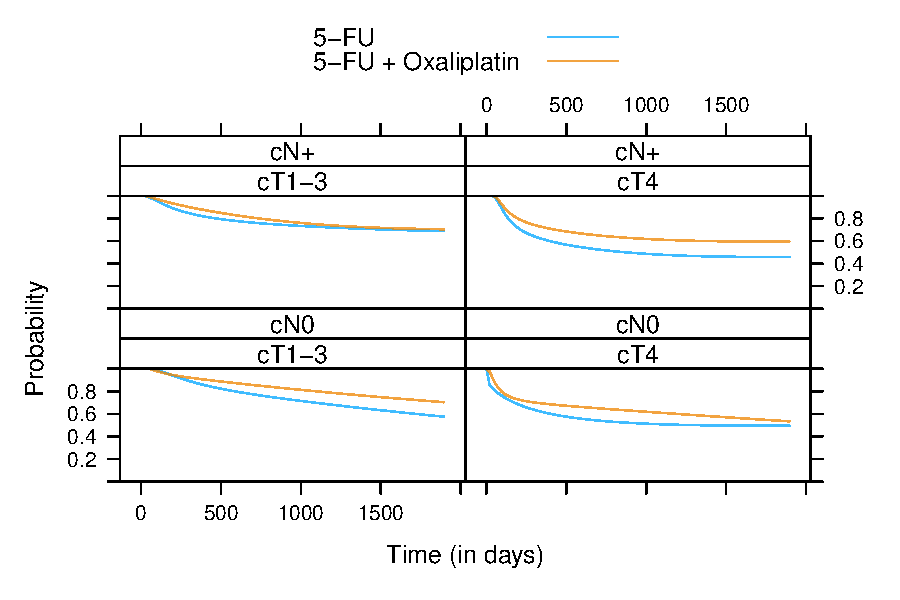
\includegraphics{figure/mtram-CAO-plot-1} 

}

\end{Schunk}
\caption{Rectal cancer: Distribution of disease-free survival times for two
         treatments in the four strata defined by lymph node involvement
         (negative or positive) and tumor grading (T1-3 or T4). \label{fig:CAO}}
\end{figure}

The implementation of marginally interpretable
linear transformation models is currently not able to
deal with mixed exact and censored outcomes in the same cluster. We
therefore recode exact event times as being interval-censored by adding a
4-day window to each exact event time (variable \code{iDFS2}).

\begin{Schunk}
\begin{Sinput}
R> ### convert "exact" event dates to interval-censoring (+/- one day)
R> tmp <- CAOsurv$iDFS
R> exact <- tmp[,3] == 1 
R> tmp[exact,2] <- tmp[exact,1] + 2
R> tmp[exact,1] <- pmax(tmp[exact,1] - 2, 0)
R> tmp[exact,3] <- 3
R> CAOsurv$iDFS2 <- tmp
\end{Sinput}
\end{Schunk}

We start with the random intercept model
\begin{eqnarray*}
\Prob(\rY > \ry \mid \text{treatment}) = 
\exp\left(-\exp\left(\frac{\eparm_1 + \eparm_2 \log(\ry) - 
                     \eshiftparm_\text{5-FU + Ox}}{\sqrt{\gamma_1^2 + 1}}\right)\right)
\end{eqnarray*}
assuming a marginal Weibull model whose effects are scaled depending on the
variance $\gamma_1^2$ of a block-specific (interaction of lymph node involvement,
tumor grading, and study center) random intercept:
\begin{Schunk}
\begin{Sinput}
R> CAO_SR <- Survreg(iDFS2 ~ randarm, data = CAOsurv)
R> CAO_SR_mtram <- mtram(CAO_SR, ~ (1 | Block), data = CAOsurv,
+                        Hessian = TRUE)
R> logLik(CAO_SR_mtram)
\end{Sinput}
\begin{Soutput}
'log Lik.' -2081.542 (df=4)
\end{Soutput}
\begin{Sinput}
R> (cf <- coef(CAO_SR_mtram))
\end{Sinput}
\begin{Soutput}
              (Intercept)                log(iDFS2) 
               -6.2990054                 0.7412855 
randarm5-FU + Oxaliplatin                    gamma1 
                0.2328600                 0.1683613 
\end{Soutput}
\begin{Sinput}
R> (OR <- exp(-cf["randarm5-FU + Oxaliplatin"] / sqrt(cf["gamma1"]^2 + 1)))
\end{Sinput}
\begin{Soutput}
randarm5-FU + Oxaliplatin 
                 0.794829 
\end{Soutput}
\end{Schunk}
We are, of course, interested in the marginal treatment effect, that is, the
hazards ratio 
%
\begin{eqnarray*}
\exp\left(-\eshiftparm_\text{5-FU + Ox} / \sqrt{\gamma_1^2 + 1}\right).
\end{eqnarray*}
%
We simply sample from the joint normal distribution of the maximum likelihood estimators
$\hat{\eparm}_1, \hat{\eparm}_2, \hat{\eshiftparm}_\text{5-FU + Ox},
\hat{\gamma}_1$ and compute confidence intervals for the marginal treatment
effect $0.79$ as
\begin{Schunk}
\begin{Sinput}
R> S <- solve(CAO_SR_mtram$Hessian)
R> # sqrt(diag(S))
R> rbeta <- rmvnorm(10000, mean = coef(CAO_SR_mtram), 
+                   sigma = S)
R> s <- rbeta[, ncol(rbeta)]
R> rbeta <- rbeta[, -ncol(rbeta)] / sqrt(s^2 + 1)
R> quantile(exp(-rbeta[, ncol(rbeta)]), prob = c(.025, .5, .975))
\end{Sinput}
\begin{Soutput}
     2.5%       50%     97.5% 
0.6473365 0.7954368 0.9848803 
\end{Soutput}
\end{Schunk}

In a next step, we stratify with respect to lymph node involvement and tumor
grading: For each of the four strata, the parameters $\eparm_1$ and
$\eparm_2$ are estimated separately:
\begin{Schunk}
\begin{Sinput}
R> CAO_SR_2 <- Survreg(iDFS2 | 0 + strat_n:strat_t ~ randarm, data = CAOsurv)
R> CAO_SR_2_mtram <- mtram(CAO_SR_2, ~ (1 | Block), data = CAOsurv,
+                          Hessian  = TRUE)
R> logLik(CAO_SR_2_mtram)
\end{Sinput}
\begin{Soutput}
'log Lik.' -2067.797 (df=10)
\end{Soutput}
\begin{Sinput}
R> (cf <- coef(CAO_SR_2_mtram))
\end{Sinput}
\begin{Soutput}
(Intercept):strat_ncN0:strat_tcT1-3  log(iDFS2):strat_ncN0:strat_tcT1-3 
                         -7.8833653                           0.9584499 
(Intercept):strat_ncN+:strat_tcT1-3  log(iDFS2):strat_ncN+:strat_tcT1-3 
                         -6.2225174                           0.7198965 
  (Intercept):strat_ncN0:strat_tcT4    log(iDFS2):strat_ncN0:strat_tcT4 
                         -3.0467542                           0.3711277 
  (Intercept):strat_ncN+:strat_tcT4    log(iDFS2):strat_ncN+:strat_tcT4 
                         -4.8207089                           0.6214653 
          randarm5-FU + Oxaliplatin                              gamma1 
                          0.2240023                           0.1474685 
\end{Soutput}
\begin{Sinput}
R> (OR_2 <- exp(-cf["randarm5-FU + Oxaliplatin"] / sqrt(cf["gamma1"]^2 + 1)))
\end{Sinput}
\begin{Soutput}
randarm5-FU + Oxaliplatin 
                0.8012313 
\end{Soutput}
\end{Schunk}
The corresponding confidence interval for the marginal treatment effect is
then
\begin{Schunk}
\begin{Soutput}
     2.5%       50%     97.5% 
0.6496110 0.8021291 0.9830439 
\end{Soutput}
\end{Schunk}
We now relax the Weibull assumption in the Cox model
\begin{eqnarray*}
\Prob(\rY > \ry \mid \text{treatment}) = 
\exp\left(-\exp\left(\frac{\basisy(\log(\ry))^\top \parm + 
                     \eshiftparm_\text{5-FU + Ox}}{\sqrt{\gamma_1^2 + 1}}\right)\right)
\end{eqnarray*}
(note the positive sign of the treatment effect).
\begin{Schunk}
\begin{Sinput}
R> CAO_Cox_2 <- Coxph(iDFS2 | 0 + strat_n:strat_t ~ randarm, data = CAOsurv, 
+                     support = c(1, 1700), log_first = TRUE, order = 4)
R> logLik(CAO_Cox_2)
\end{Sinput}
\begin{Soutput}
'log Lik.' -2021.878 (df=21)
\end{Soutput}
\begin{Sinput}
R> CAO_Cox_2_mtram <- mtram(CAO_Cox_2, ~ (1 | Block), data = CAOsurv, 
+                           Hessian = TRUE)
R> logLik(CAO_Cox_2_mtram)
\end{Sinput}
\begin{Soutput}
'log Lik.' -2025.516 (df=22)
\end{Soutput}
\begin{Sinput}
R> coef(CAO_Cox_2_mtram)
\end{Sinput}
\begin{Soutput}
Bs1(iDFS2):strat_ncN0:strat_tcT1-3 Bs2(iDFS2):strat_ncN0:strat_tcT1-3 
                     -6.374623e+01                      -2.692811e+00 
Bs3(iDFS2):strat_ncN0:strat_tcT1-3 Bs4(iDFS2):strat_ncN0:strat_tcT1-3 
                     -2.635696e+00                      -2.632237e+00 
Bs5(iDFS2):strat_ncN0:strat_tcT1-3 Bs1(iDFS2):strat_ncN+:strat_tcT1-3 
                     -7.358348e-01                      -2.515319e+01 
Bs2(iDFS2):strat_ncN+:strat_tcT1-3 Bs3(iDFS2):strat_ncN+:strat_tcT1-3 
                     -4.738795e+00                      -3.962107e+00 
Bs4(iDFS2):strat_ncN+:strat_tcT1-3 Bs5(iDFS2):strat_ncN+:strat_tcT1-3 
                     -1.489242e+00                      -9.786615e-01 
  Bs1(iDFS2):strat_ncN0:strat_tcT4   Bs2(iDFS2):strat_ncN0:strat_tcT4 
                     -2.917610e+00                      -2.681934e+00 
  Bs3(iDFS2):strat_ncN0:strat_tcT4   Bs4(iDFS2):strat_ncN0:strat_tcT4 
                     -2.214111e+00                      -5.892088e-01 
  Bs5(iDFS2):strat_ncN0:strat_tcT4   Bs1(iDFS2):strat_ncN+:strat_tcT4 
                     -4.006982e-01                      -3.998171e+01 
  Bs2(iDFS2):strat_ncN+:strat_tcT4   Bs3(iDFS2):strat_ncN+:strat_tcT4 
                     -2.373470e+00                      -1.500753e+00 
  Bs4(iDFS2):strat_ncN+:strat_tcT4   Bs5(iDFS2):strat_ncN+:strat_tcT4 
                     -4.662989e-01                       6.844420e-09 
         randarm5-FU + Oxaliplatin                             gamma1 
                     -2.454812e-01                       2.534131e-01 
\end{Soutput}
\end{Schunk}
with confidence interval
\begin{Schunk}
\begin{Soutput}
     2.5%       50%     97.5% 
0.6475265 0.7865889 0.9587480 
\end{Soutput}
\end{Schunk}
For the marginally interpretable models that can be derived from model
\code{CAO\_Cox\_2\_mtram} we can compute the probabilistic index.
This value is the meaning that over all study centers, a randomly selected patient 
receiving Oxaliplatin has a $56\%$ probability of staying disease-free
longer than a randomly
selected patient receiving the standard treatment only, given that they both 
have the same lymph node state and tumor grading.
\begin{Schunk}
\begin{Sinput}
R> nd <- CAOsurv[1:2, ]
R> tmp <- CAO_Cox_2
R> tmp$coef <- coef(CAO_Cox_2_mtram)[-22] / sqrt(coef(CAO_Cox_2_mtram)[22]^2 + 1)
R> (CAO_Cox_PI <- PI(tmp, newdata = nd[2, ], reference = nd[1, ],
+                    one2one = TRUE, conf.level = .95))[1, ]
\end{Sinput}
\begin{Soutput}
 Estimate       lwr       upr 
0.5592107 0.5072277 0.6099271 
\end{Soutput}
\end{Schunk}
but we can compute the same manually as follows:
\begin{Schunk}
\begin{Sinput}
R> ci_man <- quantile(-rbeta[, ncol(rbeta)], prob = c(.025, .5, .975))
R> (CAO_Cox_PIm <- PI(ci_man, link = "minimum extreme value"))
\end{Sinput}
\begin{Soutput}
     2.5%       50%     97.5% 
0.5105302 0.5597259 0.6069705 
\end{Soutput}
\end{Schunk}
We can fit mixed-effects transformation models 
\citep{tamasi2021tramme,Tamasi_Crowther_Puhan_2022} as follows:
\begin{Schunk}
\begin{Sinput}
R> CAO_Cox_2_tramME <- CoxphME(iDFS2 | 0 + strat_n:strat_t ~ randarm + (1 | Block), 
+                              data = CAOsurv, log_first = TRUE)
\end{Sinput}
\end{Schunk}
From this conditional model, we can obtain the conditional hazard ratio with
confidence interval:
\begin{Schunk}
\begin{Sinput}
R> exp(coef(CAO_Cox_2_tramME))
\end{Sinput}
\begin{Soutput}
randarm5-FU + Oxaliplatin 
                0.7906073 
\end{Soutput}
\begin{Sinput}
R> exp(confint(CAO_Cox_2_tramME, parm = "randarm5-FU + Oxaliplatin", 
+              estimate = TRUE))
\end{Sinput}
\begin{Soutput}
                                lwr       upr       est
randarm5-FU + Oxaliplatin 0.6406382 0.9756832 0.7906073
\end{Soutput}
\end{Schunk}
which is similar to the one of the marginally interpretable model.

% For both the mixed-effects transformation model and the marginally interpretable
% transformation model, the estimated variance parameter $\gamma_1$ is not very large,
% meaning that




% Because the estimated variance parameter $\gamma_1$ is not very large, we
% would expect to see similar results in a conditional Cox model with normal
% frailty term




\section{Assessment of Unexplained Variability}



\cite{Pollet2009} reported on an association between partner wealth and
female self-reported orgasm frequency.  It was later
pointed out \citep{Herberich+Hothorn+Nettle+Pollet2010} that the finding was
due to an incorrectly implemented variable selection procedure based on a
proportional odds (cumulative logit) model for the ordinal variable
corresponding to the question ``When having sex with your current partner,
how often did you have orgasm?'' with possible answer categories $\ry_1 =
\text{Always}$, $\ry_2 = \text{Often}$, $\ry_3 = \text{Sometimes}$, $\ry_4 =
\text{Rarely}$, or $\ry_5 = \text{Never}$.  The full model explains the
conditional distribution of orgasm frequency by $\rx = $ partner income,
partner height, the duration of the relationship, the respondents age, the
difference between both partners regarding education and wealth, the
respondents education, health, happiness, and place of living (regions in
China) of the form
%
\begin{eqnarray*}
\Prob(\text{orgasm} \le \ry_k \mid \rx) = \expit(\eparm_k + 
                                                       \rx^\top \shiftparm)
\end{eqnarray*}
%
for $i = 1, \dots, N = 1531$ independent heterosexual 
couples. In this model, the threshold parameters $\eparm_1,
\dots, \eparm_4$ are monotonically increasing and independent of $\rx$,
which implies the proportional odds property, and the regression coefficients 
$\shiftparm$ can be interpreted as log-odds ratios. We question the appropriateness of this
model here by including a subject-specific random intercept with standard
deviation $\gamma_1$. This gives rise to the marginal model
\begin{eqnarray*}
\Prob(\text{orgasm} \le \ry_k \mid \rx) = \expit \left(
\frac{\eparm_k + \rx^\top
  \shiftparm}{\sqrt{\gamma_1^2 + 1}} \right).
\end{eqnarray*}
A value of $\gamma_1$ close to zero corresponds to marginal distributions
very similar to the proportional odds model and, consequently, it is
appropriate to interpret $\shiftparm$ as log-odds ratios. Larger values of
$\gamma_1$ indicate a more variable distribution and thus the choice $\pZ =
\expit$ might be questionable.
\THcite{McLain and Ghosh}{McLain_Ghosh_2013} used a
differently parameterised link function $\pZ$ and pointed to an equivalent
interpretation as unobserved heterogeneity. 

We obtain
\begin{Schunk}
\begin{Sinput}
R> CHFLS_Polr <- Polr(orgasm ~ AincomeSD + AheightSD + RAdurationSD + 
+                     RageSD + edudiffSD + wealthdiffSD + Redu + 
+                     Rhealth + Rhappy + Region, data = orgAcc)
R> logLik(CHFLS_Polr)
\end{Sinput}
\begin{Soutput}
'log Lik.' -1852.615 (df=27)
\end{Soutput}
\begin{Sinput}
R> orgAcc$ID <- factor(1:nrow(orgAcc))
R> CHFLS_mtram <- mtram(CHFLS_Polr, ~ (1 | ID), 
+                       data = orgAcc)
R> logLik(CHFLS_mtram)
\end{Sinput}
\begin{Soutput}
'log Lik.' -1852.782 (df=28)
\end{Soutput}
\begin{Sinput}
R> coef(CHFLS_mtram)
\end{Sinput}
\begin{Soutput}
         orgasm1          orgasm2          orgasm3          orgasm4 
     -3.36220158      -1.52881197       1.38087043       3.56294225 
       AincomeSD        AheightSD     RAdurationSD           RageSD 
      0.02869432      -0.02211786       0.09097009      -0.40303118 
       edudiffSD     wealthdiffSD         Redujcol        Reduupmid 
     -0.19652655      -0.03951236       0.15395450       0.19396530 
      Redulowmid      Reduprimary     Redunoschool  Rhealthnot good 
     -0.48578975      -1.08545321      -2.03959231       1.50402662 
     Rhealthfair      Rhealthgood Rhealthexcellent    Rhappynot too 
      1.88166459       2.04364883       2.07163249       0.30627395 
Rhappyrelatively       Rhappyvery  RegionNortheast      RegionNorth 
      0.83360135       1.13098151       0.45463373       0.22429881 
   RegionInlandS   RegionCoastalE   RegionCoastalS           gamma1 
      0.55211015       0.22026234       0.65568781       0.52119277 
\end{Soutput}
\end{Schunk}
% and from $\hat{\gamma}_1 = round(coef(CHFLS_mtram)["gamma1"], 3)$ 
% can conclude that the proportional odds model is appropriate here.

With $\hat{\gamma}_1 = 0.521$ 
and almost identical log-likelihoods for both models ($-1852.615$ without
and $-1852.829$ with variance parameter $\gamma_1$), the amount of
unexplained variation seems negligible and interpretation of the effects
as log-odds ratios is appropriate.

\bibliography{mlt,packages}

\newpage

\appendix

\section{Simulations}




\subsection{Binary probit models}

With this example we want to compare the performance of \code{mtram} to the
one of \code{glmer} from package \pkg{lme4} with Laplace approximation and with
Adaptive Gauss-Hermite Quadrature with 20 nodes, and \code{glmmTMB} from package
\pkg{glmmTMB} \citep{pkg:glmmTMB}. 

For these simulations, we consider 100 clusters of size 5.
and variance $\tau = \sqrt{3}/\pi$ and $\shiftparm = (-0.5, 0, 1, 2)^\top$.
We simulate data according to the following procedure, estimate the
relevant models and repeat this 100 times.

In Figure~\ref{fig:sim-BP} we show the resulting coefficients. We can see that
all functions performed similarly in estimating the coefficienty.

\begin{Schunk}
\begin{Sinput}
R> N <- 100 # number of clusters
R> Ni <- 5  # size of clusters
R> cls <- gl(N, Ni)
R> tau <- sqrt(3)/pi
R> p <- 3
R> beta <- c(-.5, 0, 1, 2)
R> 
R> x <- cbind(1, matrix(runif(N * Ni * 3), ncol = p))
R> prb <- pnorm(x %*% beta + rnorm(N, sd = tau)[cls])
R> y <- factor(rbinom(nrow(x), size = 1, prob = prb))
R> d <- data.frame(y = y, x[,-1], cls = cls)
\end{Sinput}
\end{Schunk}




\begin{figure}[t]
\begin{Schunk}


{\centering \includegraphics{figure/sim-BP_plot-1} 

}

\end{Schunk}
\caption{Simulated binary probit data: estimated coefficients obtained by
fitting models through \code{glmer}
(Adaptive Gauss-Hermite Quadrature and Laplace approximation), \code{glmmTMB} and
exact discrete maximum-likelihood estimation with \code{mtram}.
The red dashed lines indicate the true values of the coefficients.
\label{fig:sim-BP}}
\end{figure}





\subsection{Continuous response}
We report the simulation studies conducted to assess the performance of
mixed-effects models and marginally interpretable linear transformation models
in cases where the model is misspecified with respect to the data generating 
process.

For all simulations, we consider 100 clusters of size 5.
and variance $\tau = \sqrt{3}/\pi$ and $\shiftparm = (0, 1, 2)^\top$.


We consider the following scenarios in the data generating process of a continuous
response:
\begin{enumerate}
\item We simulate from a transformation model with inverse link function
      $F = \pN$. In this setting, the conditional transformation model and the
      marginally interpretable linear transformation coincide, so we expect the models 
      fitted through \code{tramME} and \code{mtram} to have identical
      coefficients.
\begin{Schunk}
\begin{Sinput}
R> N <- 100 # number of clusters
R> Ni <- 5  # size of clusters
R> cls <- gl(N, Ni)
R> tau <- sqrt(3)/pi
R> p <- 3
R> beta <- c(0, 1, 2)
R> 
R> x <- matrix(runif(N * Ni * 3), ncol = p)
R> y <- qlogis(pnorm(x %*% beta + rnorm(N, sd = tau)[cls] + rnorm(nrow(x))))
R> ##   ^^^^^^^^^^^^^ <- h^{-1}
R> d <- data.frame(y = y, x, cls = cls)
\end{Sinput}
\end{Schunk}
      
\item We simulate from a conditional transformation model with inverse link 
      function $F = \expit$. In this setting, the model fitted through 
      \code{tramME}, which reflects the data generating process,
      should outperform the model fitted through \code{mtram}.
\begin{Schunk}
\begin{Sinput}
R> x <- matrix(runif(N * Ni * 3), ncol = p)
R> y <- qt(plogis(x %*% beta + rnorm(N, sd = tau)[cls] + rlogis(nrow(x))), df = 3)
R> ##   ^^^^^^^^^^ <- h^{-1}
R> d <- data.frame(y = y, x, cls = cls)
\end{Sinput}
\end{Schunk}
      
\item We simulate from a marginally interpretable transformation model with inverse link 
      function $F = \expit$. In this setting, we expect the model fitted
      through \code{mtram}, which reflects the data generating process,
      to outperform the model fitted through \code{tramME}.
\begin{Schunk}
\begin{Sinput}
R> Ui <- matrix(1, ncol = 1, nrow = Ni)
R> S <- tau^2
R> Sigma <- S * tcrossprod(Ui) + diag(Ni)
R> D <- diag(sqrt(diag(Sigma)))
R> Z <- rmvnorm(N, sigma = Sigma)
R> x <- matrix(runif(N * Ni * 3), ncol = p)
R> h1 <- function(x) qt(plogis(x), df = 3)
R> # ^^ <- h^{-1}
R> y <- h1(c(D %*% qlogis(pnorm(solve(D) %*% t(Z)))) + x %*% beta)
R> d <- data.frame(y = y, x, cls = cls)
\end{Sinput}
\end{Schunk}
      
\end{enumerate}

The results can be seen in Figures~\ref{fig:sim-probit_c},
\ref{fig:sim-tramME_c} and \ref{fig:sim-mtram_c}.



\begin{figure}
\begin{Schunk}


{\centering \includegraphics{figure/sim-probit_c_plot-1} 

}

\end{Schunk}
\caption{Simulated continuous data from a transformation model with $F = \pN$. 
We expect the coefficients obtained through \code{mtram} and \code{tramME} to
coincide.
The red dashed lines indicate the true values of the coefficients.
\label{fig:sim-probit_c}}
\end{figure}



\begin{figure}
\begin{Schunk}


{\centering \includegraphics{figure/sim-tramME_c_plot-1} 

}

\end{Schunk}
\caption{Simulated continuous data from a conditional model with $F = \expit$.
We expect \code{tramME} to outperform \code{mtram}.
The red dashed lines indicate the true values of the coefficients.
\label{fig:sim-tramME_c}}
\end{figure}



\begin{figure}
\begin{Schunk}


{\centering \includegraphics{figure/sim-mtram_c_plot-1} 

}

\end{Schunk}
\caption{Simulated continuous data from a marginally interpretable transformation
model with $F = \expit$.
We expect \code{mtram} to outperform \code{tramME}.
The red dashed lines indicate the true values of the coefficients. 
\label{fig:sim-mtram_c}}
\end{figure}


\subsection{Interval-censored response}
The continuous response simulated in this way can be readily converted to an
interval-censored response as follows:
\begin{Schunk}
\begin{Sinput}
R> d$yS <- Surv(floor(y), ceiling(y), type = "interval2")
\end{Sinput}
\end{Schunk}
or, for a smaller interval
\begin{Schunk}
\begin{Sinput}
R> d$yS <- Surv(floor(10*y)/10, ceiling(10*y)/10, type = "interval2")
\end{Sinput}
\end{Schunk}



\subsubsection{Intervals of length 1}

The results using the first version of the interval censoring (that is, intervals
of length 1) can be seen in Figures~\ref{fig:sim-probit_IC1}, 
\ref{fig:sim-tramME_IC1}, \ref{fig:sim-mtram_IC1}.



\begin{figure}
\begin{Schunk}


{\centering \includegraphics{figure/sim-probit_IC1_plot-1} 

}

\end{Schunk}
\caption{Simulated interval-censored data (interval of length 1)
from a transformation model with $F = \pN$. 
We expect the coefficients obtained through \code{mtram} and \code{tramME} to
coincide.
The red dashed lines indicate the true values of the coefficients.
\label{fig:sim-probit_IC1}}
\end{figure}



\begin{figure}
\begin{Schunk}


{\centering \includegraphics{figure/sim-tramME_IC1_plot-1} 

}

\end{Schunk}
\caption{Simulated interval-censored data (interval of length 1)
from a conditional model with $F = \expit$.
We expect \code{tramME} to outperform \code{mtram}.
The red dashed lines indicate the true values of the coefficients.
\label{fig:sim-tramME_IC1}}
\end{figure}



\begin{figure}
\begin{Schunk}


{\centering \includegraphics{figure/sim-mtram_IC1_plot-1} 

}

\end{Schunk}
\caption{Simulated interval-censored data (interval of length 1)
from a marginally interpretable transformation
model with $F = \expit$.
We expect \code{mtram} to outperform \code{tramME}.
The red dashed lines indicate the true values of the coefficients.
\label{fig:sim-mtram_IC1}}
\end{figure}


\subsubsection{Intervals of length $0.1$}

The results using the first version of the interval censoring (that is, intervals
of length 0.1) can be seen in Figures~\ref{fig:sim-probit_IC10}, 
\ref{fig:sim-tramME_IC10}, \ref{fig:sim-mtram_IC10}.




\begin{figure}
\begin{Schunk}


{\centering \includegraphics{figure/sim-probit_IC10_plot-1} 

}

\end{Schunk}
\caption{Simulated interval-censored data (interval of length $0.1$)
from a transformation model with $F = \pN$. 
We expect the coefficients obtained through \code{mtram} and \code{tramME} to
coincide.
The red dashed lines indicate the true values of the coefficients. 
\label{fig:sim-probit_IC10}}
\end{figure}



\begin{figure}
\begin{Schunk}


{\centering \includegraphics{figure/sim-tramME_IC10_plot-1} 

}

\end{Schunk}
\caption{Simulated interval-censored data (interval of length $0.1$)
from a conditional model with $F = \expit$.
We expect \code{tramME} to outperform \code{mtram}.
The red dashed lines indicate the true values of the coefficients.
\label{fig:sim-tramME_IC10}}
\end{figure}



\begin{figure}
\begin{Schunk}


{\centering \includegraphics{figure/sim-mtram_IC10_plot-1} 

}

\end{Schunk}
\caption{Simulated interval-censored data (interval of length $0.1$)
from a marginally interpretable transformation
model with $F = \expit$.
We expect \code{mtram} to outperform \code{tramME}.
The red dashed lines indicate the true values of the coefficients.
\label{fig:sim-mtram_IC10}}
\end{figure}


%<<mtram-mlt-coef, echo = FALSE, results = "hide">>= 
%### print coefs for regression tests
%objs <- ls()
%mltobj <- objs[grep("^mlt_", objs)]
%sapply(mltobj, function(m) eval(parse(text = paste("coef(", m, ")"))))
%@





\end{document}

